% XeLaTeX can use any Mac OS X font. See the setromanfont command below.
% Input to XeLaTeX is full Unicode, so Unicode characters can be typed directly into the source.

% The next lines tell TeXShop to typeset with xelatex, and to open and save the source with Unicode encoding.

%!TEX TS-program = xelatex
%!TEX encoding = UTF-8 Unicode

\documentclass[a4paper,promaster]{ructhesis}

%自添宏包
\usepackage{skak}%国际象棋
\usepackage{subfigure}%子图http://www.ctex.org/documents/latex/graphics/node111.html
\usepackage{chemfig}%化学式
\usetikzlibrary{trees}
\usepackage{hyperref}
\usepackage{algorithm}
\usepackage{algorithmicx}
\usepackage{algpseudocode}
\usepackage{float}
\usepackage{makecell}
\usepackage{listings}
\usepackage{xcolor}
\usepackage{threeparttable}

\usepackage[section]{placeins}
\usepackage{url}
\usepackage[backend=biber,bibstyle=gb7714-2015,gbnamefmt=lowercase,gbpub=false]{biblatex}
\addbibresource{ref/test.bib}
\newcommand{\upcite}[1]{\textsuperscript{\textsuperscript{\cite{#1}}}}

\usepackage{notoccite}

\hypersetup{
    colorlinks=true,            % 激活链接颜色,去掉链接边框
    linkcolor=black,              % 文档内部链接颜色(如图表等引用)
    citecolor=black,            % 文献引用链接颜色
    filecolor=black,   % 文件链接颜色
    urlcolor=black            % 外部URL链接颜色
}

% list figure and table name
\renewcommand{\listfigurename}{图目录}
\renewcommand{\listtablename}{表目录}

\floatname{algorithm}{算法}
\counterwithin{algorithm}{chapter}

\renewcommand{\algorithmicrequire}{\textbf{输入:}}
%Use Input in the format of Algorithm
\renewcommand{\algorithmicensure}{\textbf{输出:}}
%UseOutput in the format of Algorithm
\algnewcommand\algorithmicforeach{\textbf{for each}}
\algdef{S}[FOR]{ForEach}[1]{\algorithmicforeach\ #1\ \algorithmicdo}
%将封面信息补全,相关专业名称过长的请在文字前添加命令\ziju{-0.15}
%文头
% \sign{中国人民大学本科毕业论文}
\sign{专业硕士学位论文}
%\sign{博士学位论文}



%以下信息本科研究生都需要补全
\title{基于近存计算技术的矩阵向量乘优化研究}%论文题名
\author{张魁耀辉}%作者
\school{信息学院}%学院
\field{大数据技术与工程}%专业
\studentid{2023103756}%学号
\advisor{王晶}%指导老师
\date{2025年05月01日}


%以下本科填写
\grade{}%年级
\score{4.0}%成绩
\thesiscode{论文编码:RUC-BK-专业代码}%论文编码
\subtitle{}%论文副题名,没有不填写


%以下研究生填写
\etitle{\ziju{-0.2}Research on GEMV Optimization Based on Processing-in-Memory Technology}%英文题目
\keywords{近存计算;矩阵向量乘;查找表}%论文主题词
%摘要关键词
\keywordzh{近存计算 \quad 矩阵向量乘 \quad 查找表}%中文摘要关键词
\keyworden{Processing-in-Memory \qquad GEMV \qquad Lookup-Table}%英文摘要关键词

\lstset{
    language=c++, % 设置语言
	basicstyle=\ttfamily, % 设置字体族
	breaklines=true, % 自动换行
	keywordstyle=\bfseries\color{NavyBlue}, % 设置关键字为粗体,颜色为 NavyBlue
	morekeywords={}, % 设置更多的关键字,用逗号分隔
	emph={self}, % 指定强调词,如果有多个,用逗号隔开
    emphstyle=\bfseries\color{Rhodamine}, % 强调词样式设置
    commentstyle=\itshape\color{black!50!white}, % 设置注释样式,斜体,浅灰色
    stringstyle=\bfseries\color{PineGreen!90!black}, % 设置字符串样式
    columns=flexible,
    numbers=left, % 显示行号在左边
    numbersep=2em, % 设置行号的具体位置
    numberstyle=\footnotesize, % 缩小行号
    frame=single, % 边框
    framesep=1em % 设置代码与边框的距离
}

%
\begin{document}

%扉页
\maketitle

%覆盖plain页眉格式,使chapter首页也有页眉
\fancypagestyle{plain}{
	\pagestyle{fancy}
}

%独创性声明
\originality
%授权书在这插入
\authorization{figures/shouquan.png}
%中文摘要
\pagestyle{fancy}
% the abstract
\begin{abstractzh}
RUCThesis 是根据中国人民大学《本科论文指导手册》和《研究生学位论文及其摘要的撰写和印制要求》而制作的 \LaTeX\ 论文模板。
\end{abstractzh}
%英文摘要
% the abstract
\begin{abstracten}
    The successful application of Large Language Models (LLMs) in multiple domains has propelled the advancement of artificial intelligence. Nevertheless, they are plagued by drawbacks such as high computational costs and substantial memory demands. Optimizing the inference efficiency and reducing resource consumption have emerged as core issues. Mainstream LLMs adopt the Decoder-Only architecture, within which the Generalized Matrix-Vector Multiplication (GEMV) holds a dominant position in LLM inferences. Due to its inherent characteristics, GEMV constitutes a memory bounded task, with the utilization of computing-intensive hardware like GPUs being low. It has always become a system bottleneck in edge scenarios. Processing-in-Memory (PIM) represents an emerging computing paradigm capable of resolving the memory bounded problem in traditional computing architectures. Emerging PIM hardware boasts advantages such as high bandwidth, high storage capacity, high parallelism, and high energy efficiency, yet it also suffers from limitations including weak computing capabilities and significant communication overhead. How to adapt hardware acceleration from a software perspective and how to modify the design of hardware to optimize its application performance through a hardware-software co-design solution have become subjects warranting in-depth research.

    This thesis investigates the hardware-software co-design solution for GEMV based on Processing-in-Memory technology: 1) On the PIM hardware, a matrix-vector multiplication algorithm based on lookup tables is devised. Lookup tables are employed to eliminate complex computations, and memory access optimizations are implemented for the multi-level storage structure within the PIM hardware. This encompasses the lookup table blocking algorithm to reduce the number of memory accesses via DMA and the rearrangement of matrix rows and columns to minimize cache access and enhance data locality in registers. 2) On the simulator, to address the computational bottlenecks of software algorithms on real hardware, special processing unit and instructions are designed based on the cycle-accurate PIM simulator to enhance its computing capacity. This includes the fusion of table lookup and addition instructions for efficient and rapid query of products and accumulation, as well as the design of vector instructions based on lookup tables for vectorized lookup and memory access to boost computing efficiency. Finally, detailed tests were carried out on the aforementioned algorithms on three hardware platforms, namely CPU, GPU, and PIM hardware, including tests on the total throughput and energy efficiency of the GEMV operator. The experimental results indicate that the throughput of the GEMV operator on the PIM hardware amounts to 355 GOPS, approximately reaching 93\% of the theoretical performance. It is 14.7 times that of the CPU platform, and the energy efficiency is approximately 8.6 times that of the CPU platform and 1.13 times that of the GPU platform.
\end{abstracten}




\frontmatter

%正文目录
\pagenumbering{arabic}
\tableofcontents
%插图目录
{\renewcommand{\addvspace}[1]{} \listoffigures}
%表格目录
{\renewcommand{\addvspace}[1]{} \listoftables}


\mainmatter\clearpage
\pagestyle{newformat}

%正文章节
\chapter{\LaTeX{} 介绍}
%\section{安装\LaTeX{} }
%\subsection{Mac OS X}
%\begin{figure}[htbp]
%\centering\includegraphics[width=5cm,height=1.32cm]{figures/Logo_2.pdf}
%\caption[示意图]{用LaTeX画图}
%\end{figure}
\LaTeX\footnote{https://zh.wikipedia.org/wiki/LaTeX}(英语发音:/ˈleɪtɛk/ lay-tek或英语发音:/ˈlɑːtɛk/ lah-tek,音译“拉泰赫”),文字形式写作\LaTeX ,是一种基于\TeX\ 的排版系统,由美国电脑学家莱斯利·兰伯特在20世纪80年代初期开发,利用这种格式,即使用户没有排版和程序设计的知识也可以充分发挥由\TeX\ 所提供的强大功能,能在几天,甚至几小时内生成很多具有书籍质量的印刷品。对于生成复杂表格和数学公式,这一点表现得尤为突出。因此它非常适用于生成高印刷质量的科技和数学类文档。这个系统同样适用于生成从简单的信件到完整书籍的所有其他种类的文档。

\LaTeX\ 使用\TeX\ 作为它的格式化引擎,当前的版本是\LaTeX 2ε。
\begin{figure}[htbp]
\centering
\subfigure[国际象棋]{ 
	\label{fig:mini:subfig:a} %% label for first subfigure 
	\begin{minipage}[b]{0.5\textwidth} 
	\centering 
	\fenboard{%
	r5k1/%
	1b1p1ppp/%
	p7/%
	1p1Q4/%
	2p1r3/%
	PP4Pq/%
	BBP2b1P/%
	R4R1K w - - 0 20}
	\mbox{}\showboard
	\end{minipage}}% 
\subfigure[化学式]{
	\label{fig:mini:subfig:b} %% label for second subfigure 
	\begin{minipage}[b]{0.5\textwidth} 
	\centering 
      	\chemfig{
 	H_3C-[:72]{\color{blue}N}*5(- 
	*6(-(={\color{red}O})-
	{\color{blue}N}(-CH_3)-
	(={\color{red}O})-
	{\color{blue}N}(-CH_3)-=)--
	{\color{blue}N}=-)}
   	 \end{minipage}} 
\caption{\LaTeX\ 绘图示例} 
\label{fig:mini:subfig} %% label for entire figure 
\end{figure}


\chapter{相关工作}

本章节首先介绍大模型推理相关概念和工作,包括对现有流行大模型的架构和算子的介绍,对推理加速的技术尤其是模型量化的相关工作进行介绍,以及阐明推理性能和矩阵向量乘算子的关系。其次介绍近存计算的研究现状,首先介绍近存计算的发展历史以及相关工作,然后介绍第一款商用近存计算硬件UPMEM的硬件架构和特性,最后详细介绍各个领域基于UPMEM加速应用的相关工作。

\section{大模型推理介绍}

\subsection{基本概念}
自2022年11月OpenAI发布聊天机器人产品ChatGPT以来,其强大的语言理解对话能力和逻辑推理能力震惊了世界,并以势不可挡之式席卷全球,并受到了资本的热捧。其背后拥有强大智能的GPT(Generative Pre-trained Transformer)大语言模型(Large Language Model, LLM)凭借惊人的通用智能应用到了各行各业,开启了LLM时代。

GPT模型的结构源于Google在2017年提出的一个基本模型结构Transformer \cite{Transformer}。Transformer模型本身是为解决序列到序列(Seq2Seq)的自然语言翻译问题,构造了编码器(Encoder)模型用于理解待翻译序列,再使用解码器(Decoder)模型结合Encoder的理解生成翻译序列。在Encoder和Decoder中创造性地使用了自注意力(Self-Attention)机制,使得模型的性能表现异常优异,击败了当时其他的翻译模型。基于Transformer结构,自然语言处理(Natuarl Language Processing,NLP)领域的模型逐渐形成了三条不同的发展路径,分别是Encoder-Only架构、Encoder-Decoder架构和Decoder-Only架构。Encoder-Only架构的模型非常擅长做语义理解,其应用领域往往是文本分类,其中最著名的模型当属Bert\cite{Bert};Encoder-Decoder架构和Transformer的应用领域类似,主要是用在机器翻译领域,其中比较著名的模型同是Google公司的T5\cite{T5}。Bert和T5模型在前GPT时代基本确定了NLP模型的预训练+微调的部署范式:由大公司使用大量数据集训练基础通用模型(预训练模型),在此基础上由使用者自行用少量高质量数据微调模型以适应不同的下游任务。

Decoder-Only架构的模型与前面两者不同,可以直接自回归地生成自然语言,常常应用到文本续写领域和聊天机器人,其中代表模型就是OpenAI的GPT模型。最早的GPT-1\cite{GPT-1}仍然采用有监督和无监督混合训练的方式直接生成下一个词元,效果并不是很理想。到了GPT-2\cite{GPT-2},GPT模型开始使用无监督的训练方式,加大了训练数据量并提升模型参数规模到150亿,无须微调模型而只需简单地通过写提示词(Prompt)就可以达到非常好的效果。到了GPT-3\cite{GPT-3},进一步将模型参数量提升到了惊人的1750亿,并专注于提升模型的上下文学习能力(In-Context-Learning,ICL)。量变引起了质变,GPT-3的效果非常优异,为接下来的GPT3.5以及ChatGPT的爆火做了铺垫。得益于Decoder-Only架构模型在大量数据集上的良好零样本(Zero Shot)学习能力\cite{Zero-Shot}和少样本(Few Shot)微调能力\cite{Few-Shot},大模型的参数规模不断增长(从前GPT时代Bert的1.1亿参数到GPT-3的1750亿),参数量的膨胀对于大模型推理提出了严峻的挑战,大公司旗下的云计算中心需要使用集群分布式推理上千亿大模型,常见的硬件几乎无法部署推理参数量最小的70亿参数模型。

\begin{figure}[!htbp]
	\centering
    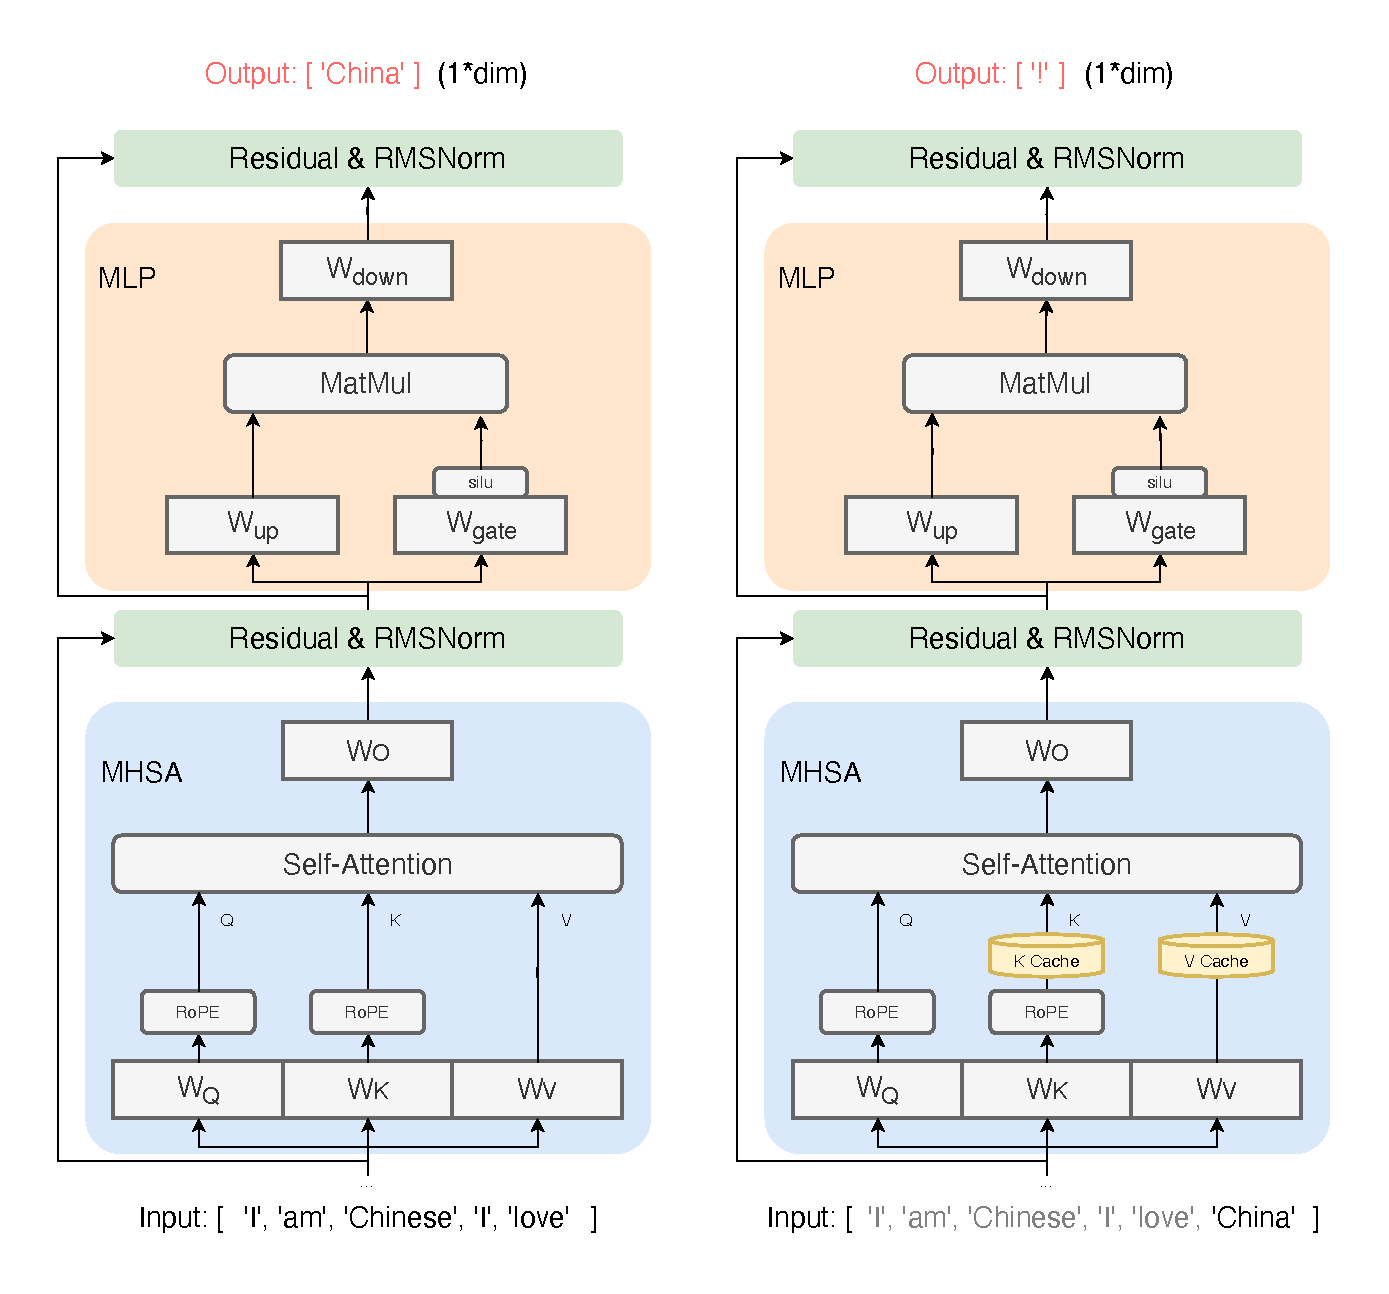
\includegraphics[width=0.9\textwidth]{figures/LLMInfer.pdf}
	\caption{现代主流大模型推理示意图。图左为Prefill阶段的单层Decoder的计算,图右为Decode阶段对应的计算}
    \label{LLMInfer}
\end{figure}

要想了解大模型在常用硬件平台上的推理瓶颈,就需要先了解大模型的结构,从开源的大模型入手是最佳选择。其中使用最广微调性能最高的开源大模型当属Facebook推出的Llama系列。Llama系列的模型架构都秉承类似的结构,以Llama2-7B\cite{Llama2}为例,模型一般由多层Decoder组成,每层Decoder分为多头注意力(Multi-Head Self-Attention,MHSA)和前馈神经网络(Feed-Forward Neural Network,FFN)两个主要部分。在LLM进行推理的时候,分为两个阶段:用户输入提示词(Prompt)进入网络到模型生成第一个词元(Token)的阶段称作预填充阶段(The Prefilling Stage),再生成了第一个token之后,LLM不断自回归生成下一个token直到输出终止符的阶段称为解码阶段(The Decoding Stage)。如图\ref{LLMInfer}所示,两个阶段执行的计算并不相同,主要体现在Self-Attention部分,预填充阶段执行的是通用矩阵矩阵乘(Generalized Matrix Multiplication,GEMM),而在解码阶段执行的是通用矩阵向量乘(Generalized Matrix Vector Multiplication,GEMV)。两者不同的原因主要在于现代Decoder-Only架构的LLM在自回归生成阶段普遍采用因果注意力(Causal Self-Attention)并通过KVCache机制减少计算量,如图\ref{KVCache}所示,因果注意力会使用因果掩码对QK乘积矩阵的上三角置0:当生成第四个token时,Query1和Key2到Key4点注意力都被掩码置0无效化,为的是防止其与未来生成的token做注意力计算以保持因果一致性。第四个token进行推理时真正的新数据就是Query4、Key4、Value4和Attention4。因而KVCache就是将K向量和V向量缓存起来,每次只需要最新生成的Query向量参与运算,减少重复的注意力计算,此时Self-Attention的计算为GEMV。

\begin{figure}[!htbp]
	\centering
    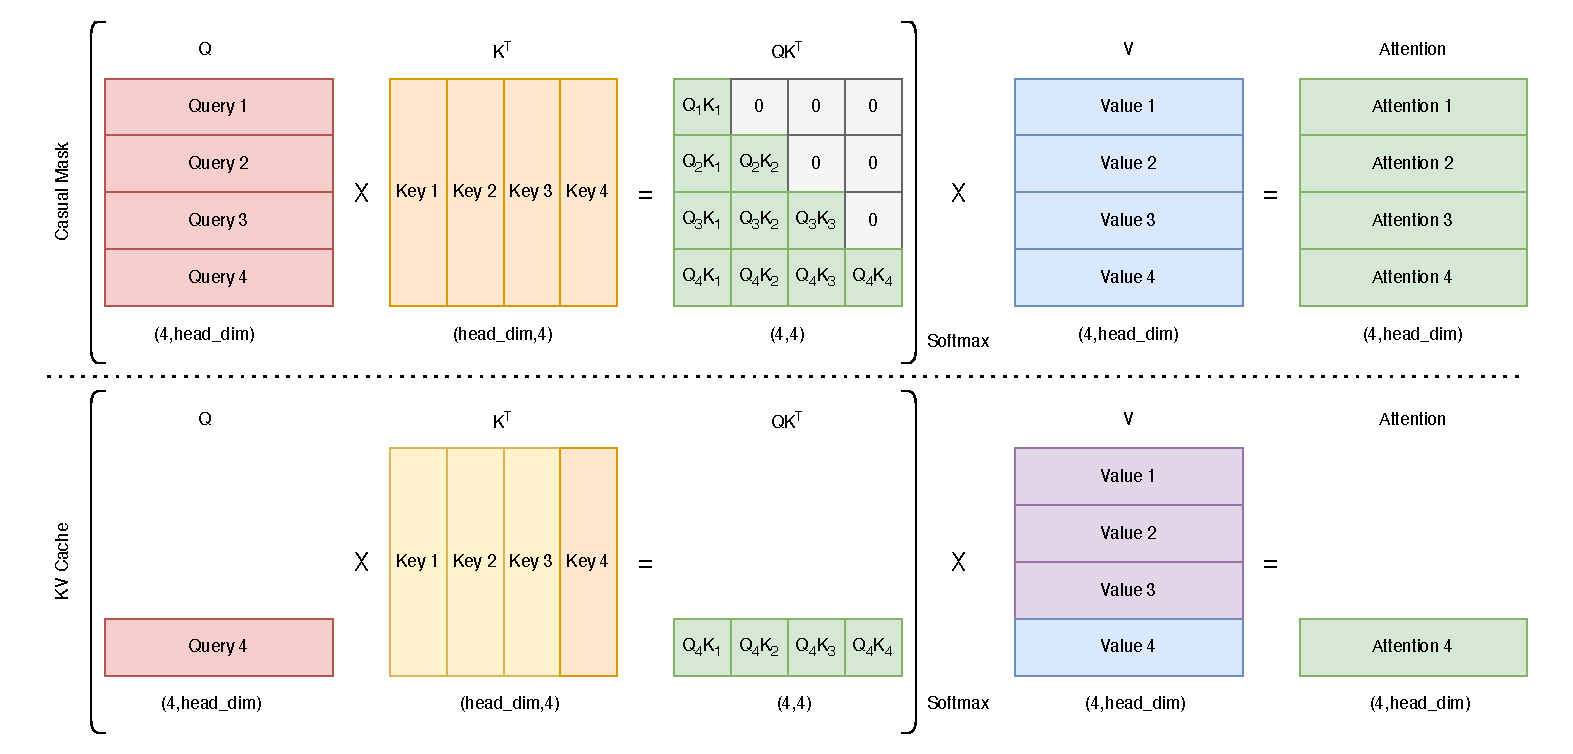
\includegraphics[width=0.9\textwidth]{figures/KVCache.pdf}
    \caption{Self-Attention计算简介。图左为Prefill阶段,使用因果掩码,图右为Decoder阶段,使用KVCache}
	\label{KVCache}
\end{figure}

大模型的推理往往表现为内存瓶颈,尤其是在用户量不多的本地或边端场景,推理中的解码阶段占据主导地位,有数据表明,解码阶段代表性算子GEMV平均占据82.3\%的GPU运行时间,而预填充阶段的代表性算子GEMM的平均耗时只占2\%,剩下的一些非线性算子总占比不到20\%;同时在执行GEMV算子时,GPU的硬件利用率显著地低于GEMM算子,并且将绝大部分的时间消耗在内存拷贝和数据传输上,表现为内存瓶颈\cite{SamsungHotChips}。这使得缓解内存数据的搬移成为大模型推理的主要性能瓶颈,针对GEMV的优化对于提升大模型的推理效率至关重要,具有重大研究价值。

\subsection{大模型量化技术}
加速大模型推理有许多手段,包括模型量化、模型压缩、矩阵稀疏化、知识蒸馏、内存管理和批处理等等技术\cite{LLMInferSurveyTsingHua},其中最流行以及能够显著降低模型的内存瓶颈的方法当属模型量化。所谓的量化就是指将模型的高bit参数(float32)通过一系列措施(最小化推理精度损失)转化为较低的位宽存储。这样做能够极大缩减模型尺寸,在硬件资源有限的情况下支持低精推理,使得本地大模型或边端大模型成为可能。以一组float32向量量化成int8向量为例,如图\ref{Quant:Norm}所示,取得这组float32向量的最大绝对值5.4,将其映射到int8的动态范围$[-128,127]$,计算得到缩放因子scale为23.5,将向量的每个元素与scale相乘并做整数舍入得到int8向量,此时完成量化;当需要量化后的向量参与计算时需要先解量化,将int8向量的每个元素与scale相除进行解量化,还原成float32向量。

\begin{figure}[htbp!]
	\centering
    
	\subfigure[正常对称量化]{
		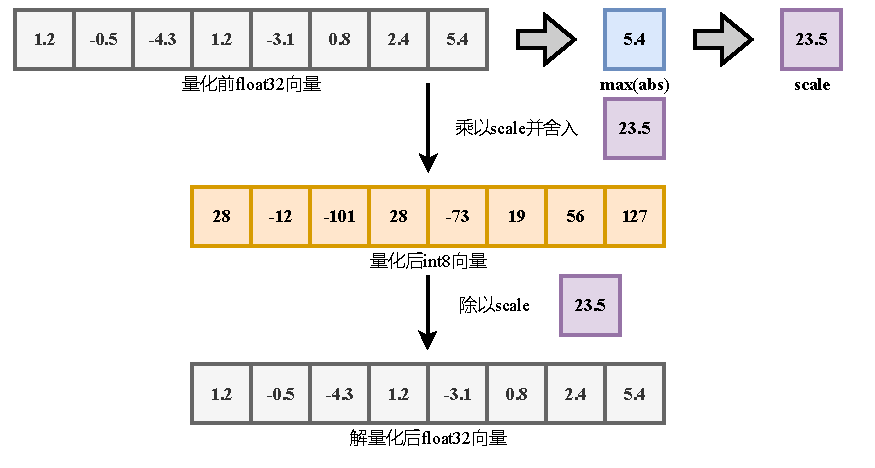
\includegraphics[width=0.9\textwidth]{figures/QuantNorm.pdf}
		\label{Quant:Norm}}
	\\
	\subfigure[含有离群值的量化]{
		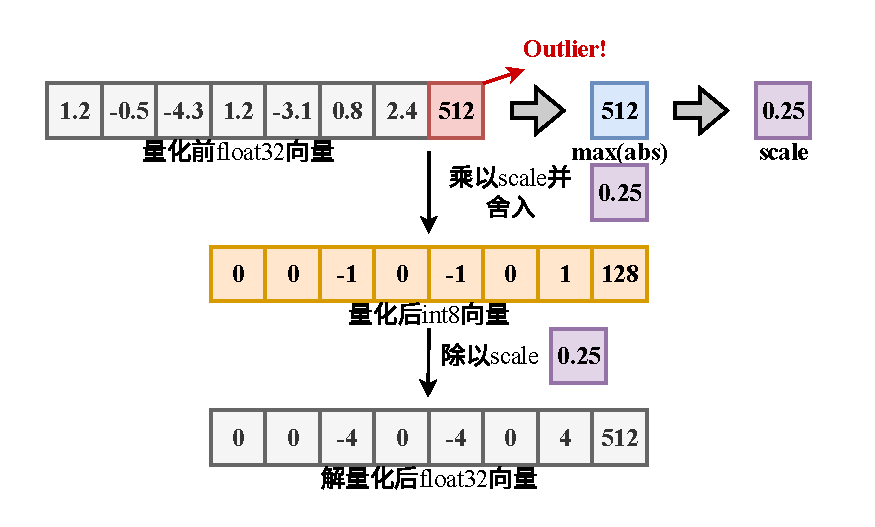
\includegraphics[width=0.9\textwidth]{figures/QuantAbnorm.pdf}
        \label{Quant:Abnorm}}
	\label{Quant}
	\caption{Float32向量对称量化为Int8向量示意图}
\end{figure}

上述量化是非常标准的对称量化:所谓对称量化就是取得原数值域的一个对称区间量化到目标数值区域,一般使用最大绝对值确定对称区间。而与之相对的非对称量化就是量化原数值域的非对称区间,使用的是最小值和最大值;对称量化是非对称量化的一种特殊情况,二者都可以用公式\ref{QuantEqu}来表示,其中r是原始浮点数,S是缩放因子scale,Z是零点偏移,q是量化后的数值。当为对称量化时,零点无偏移,$r_{max}-r_{min}=2r_{max_abs}$。量化一般采用训练后量化(Post Training Quantization,PTQ)的方式以降低量化成本(简单的数学变换或者少量校准数据集),主要的量化对象就是激活值和权重,按照上述的方式将激活和权重全部量化到8bit的量化称为W8A8(weight 8bit activation 8bit)量化。但是假如激活向量或权重矩阵中,存在一个特别大的值如图\ref{Quant:Abnorm}所示,为512,那么scale计算就得到为0.25,将原float32向量与scale相乘再舍入取整为int8,发现绝大部份数都变为了0,0在浮点数制中是一个特殊值,任何数与0相乘或相除都是0,因此将int8向量反量化后,float32向量中的大部分数据也都变为0,从而导致精度严重损失。

\begin{equation}
    q = round\left(\frac{r}{S} + Z\right), \quad S=\frac{r_{max}-r_{min}}{q_{max}-q_{min}}, \quad Z=q_{min}-\frac{r_{min}}{S}
    \label{QuantEqu}
\end{equation}

为了解决这种离群值带来的量化精度影响,许多工作提出了不同的方案。其中比较出名的int8量化方案为Dettmers等人提出的LLM.int8\cite{LLMINT8},该方法的主要思路在于离群值分布往往在特定的维度且比较稀疏,因此可以将离群值提取出来用float16进行计算,剩下的量化到int8,这样的混合精度分解能够很大程度提升量化精度。SmoothQuant采用了不同的思路\cite{SmoothQuant}做W8A8量化,其观察到当前的LLM的激活相对权重难以量化,因此提出了一种数学上等价的逐通道缩放变换,引入一个对角矩阵存放激活逐通道的缩放因子scale factor,将原激活除以对应的缩放因子作为新的激活,原矩阵等价地乘以对应的缩放因子作为新的权重,这样就能将激活中难以量化的离群值平滑到了权重当中,二者都变得容易量化了。Lin等人提出了一种W4A16的量化(仅量化权重)\cite{AWQ},其核心思想是基于激活值的分布挑选对最终结果影响较大的权重,将这些显著权重保留精度分解,剩余权重采用低bit量化,以较小的量化误差达到大幅度减少内存占用的效果。在量中同样有一类工作可以实现非常低bit的量化,即基于机器学习的量化,其中最具代表性的当属GPTQ。GPTQ本身的核心思想是对LLM进行逐层量化,希望在该层找到一个新权重(量化过后),使得其和使用老权重相比输出之间的误差尽可能小。GPTQ将这个作为训练目标使用机器学习的方式进行优化,基于此前的OBQ工作\cite{OBQ},对训练算法做了近似和加速,能够达到3-4bit的超低精度量化。Yao等人开展了一系列LLM上的量化工作:ZeroQuant系列\cite{ZeroQuant1,ZeroQuant2,ZeroQuantFP}。ZeroQuant-V1主要是针对GPU硬件构建了强大的推理后端并使用逐层知识蒸馏缓解量化带来的精度下降问题\cite{ZeroQuant1};ZeroQuant-V2则是针对常见的不同的PTQ方法进行了全面的分析,并提出了一种低秩补偿的技术来缓解量化带来的误差\cite{ZeroQuant2};ZeroQuantFP基于GPTQ的量化和低秩补偿,重点探索来浮点数据格式对于量化的影响,得出float8激活优于int8,float8权重与int8权重相当,float4权重优于int4权重的结论\cite{ZeroQuantFP}。

\subsection{矩阵向量乘算子}
GEMV作为基本的线性代数运算被广泛地使用于各种科学计算和神经网络计算当中,其本身可以视作GEMM中矩阵维度为1的一种特例。关于GEMM和GEMV的计算加速优化方法一直是研究人员的研究热点,因为GEMM和GEMV作为BLAS(Basic Linear Algebra Subprograms)中最为基本的两个,其性能的提升将极大提升建立于其基础上的应用性能。GEMM的优化主要分为两个方面,分别是数学算法上的优化和计算机系统层面的优化。前者主要是在数学算法上减少GEMM需要执行计算量,其中最经典的算法是Strassen算法\cite{Strassen},其将相乘的每个矩阵分别分解为大小相同的四个子矩阵,通过对四个子矩阵执行一系列的矩阵加法和乘法运算得到最终的乘积矩阵,成功将矩阵乘法的时间复杂度从$\O(n^3)$优化到$\O(n^{\log_{2}7})$,但是由于GEMV中向量无法进行有效地分块,因此Strassen算法无法直接应用到GEMV上的优化;另一种,也是工作最多且更加有效的优化,通过将矩阵进行合适的分块和内存布局,减少计算机在执行计算过程中的重复的和开销大的访存,增强数据的局部性。常见的工作都是根据所使用硬件的离计算核心最近的一级存储器件(比如CPU中是L1 Data Cache,GPU中CUDA的shared memory\cite{Cuda})的存储大小,对矩阵进行合适大小的分块以在执行每个小块的计算时访存都能落到最近的存储器而无需访问更低速的内存。

GEMV的常规计算方式有两种,如图\ref{GEMVBasic}所示,可以类似向量的内积和外积定义GEMV的内积和外积概念。如图\ref{GEMVBasic:Inner},GEMV的内积可以定义为向量和矩阵的一行或一列的对应元素乘积之和,结果是最终结果向量的一个元素。如图\ref{GEMVBasic:Outer},GEMV的外积可以定义为向量的某个元素与矩阵对应行或列的所有元素乘积,结果是一个向量,将所有向量对应相加得到最终结果向量。在传统CPU平台下,GEMV的内积效率更高,因为其数据局部性更好,内积的累加结果基本能够留存在寄存器中,不需要频繁读写结果向量;当然GEMV的外积在某些场景下也有用武之地。除了考虑寄存器效率外,高速缓存(Cache)的命中率也非常重要:无论是何种方式,只需要Cache容量大于矩阵的两行或两列所占的空间,命中率就会很高,如果矩阵的两行或两列所占的空间过大,则需要将矩阵或向量在某一个维度上进行分块,以达更高缓存命中率。分块后,对于大多数的存储器来说,顺序读取效率是最高的,因此需要将数据按照顺序访问的方式进行重排,称为数据打包。如\ref{GEMVBasic}所示,将矩阵按行或列分成了N块,对每一块进行数据打包依次计算。

\begin{figure}[htbp!]
	\centering
	\subfigure[GEMV内积]{
		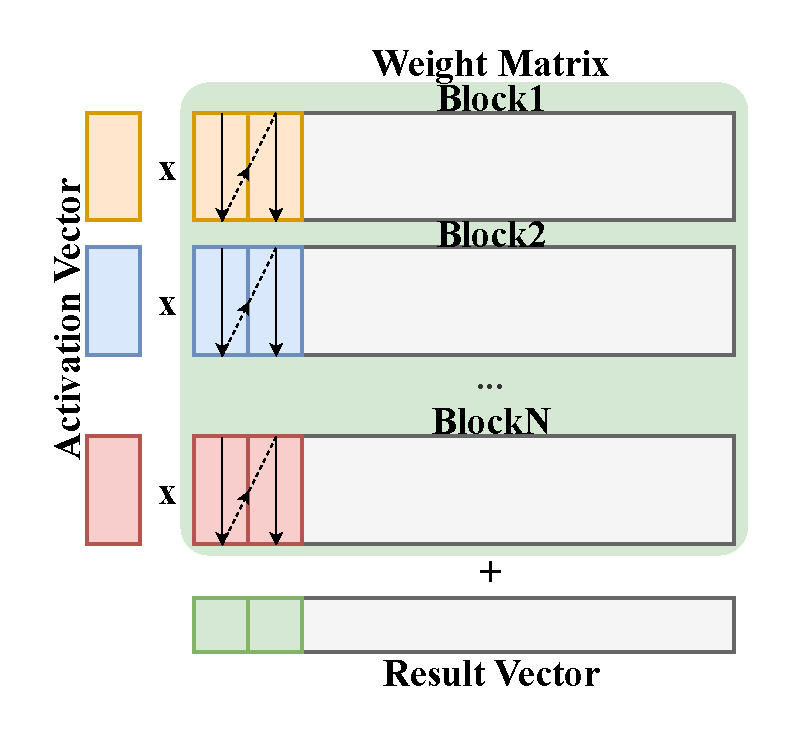
\includegraphics[width=0.43\textwidth]{figures/GEMVInner.pdf}
		\label{GEMVBasic:Inner}}
	\subfigure[GEMV外积]{
		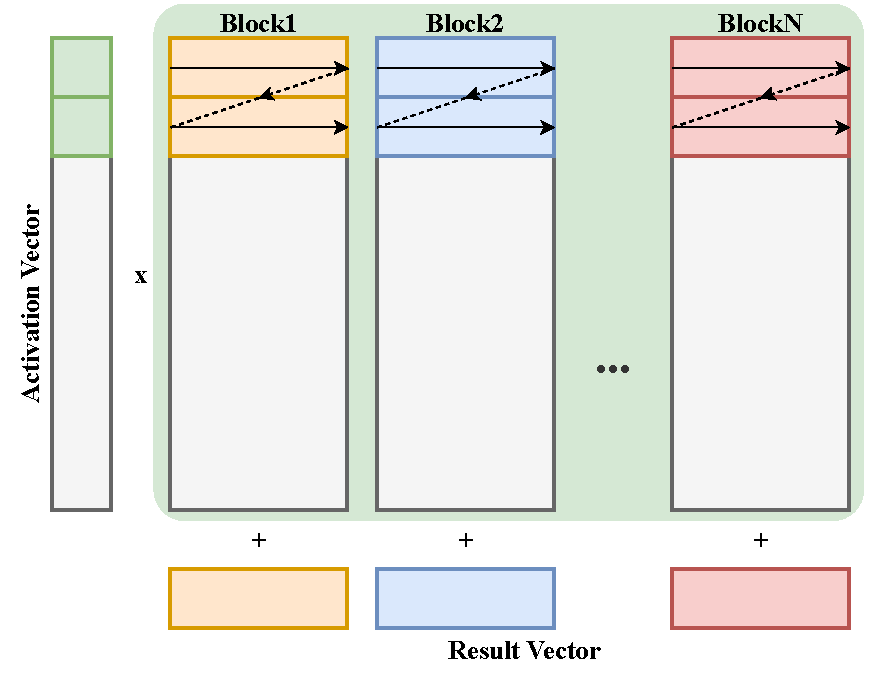
\includegraphics[width=0.47\textwidth]{figures/GEMVOuter.pdf}
        \label{GEMVBasic:Outer}}
	\label{GEMVBasic}
	\caption{GEMV基本计算和优化方法}
\end{figure}

常规的优化手段如上所述,当然还可以使用多线程进行优化,此时只需要考虑各个线程的数据划分和线程间的同步开销即可。除此之外许多相关硬件被设计并对其加速提供了支持,这其中包括基于单指令多数据(Single Instruction Multiple Data,SIMD)的Intel的向量单元和AVX指令集,可以在0.5个周期内完成512bit向量的融合乘加运算(Fused Multiply Accumulate,FMA)操作\cite{IntelAVX}。还有Nvidia基于单指令多线程(Single Instruction Multiple Threads,SIMT)模型设计的CUDA Core\cite{Cuda},以及专门用于GEMM计算的Tensor Core\cite{TensorCore}等等,都极大地提升了GEMM和GEMV的计算效率。

\section{近存计算研究现状}

\subsection{近存计算技术发展}
早在上世纪七十年代左右,近存计算的思想就已经\cite{CellularLogicInMemory,LogicInMemory}初具雏形,这时普遍提到的概念是“Logic-in-Memory”,其核心思想是在动态随机存取存储器(Dynamic Random Access Memory,DRAM)的存储单元上增加简单的逻辑电路使得DRAM本身可以进行一些简单的运算。在九十年代,Wulf等人针对处理器(CPU)和存储器(DRAM)之间不断增大的速度差异,通过科学的建模和实验进行了分析,通过系统性的分析和实验,提出了内存墙(Memory Wall)的概念以说明CPU和DRAM之间速度存在的难以逾越的鸿沟\cite{MemoryWall}。许多学者围绕该问题提出了不同的解决方案,其中,有部分学者提出存内计算(Processing in Memory, PIM)的思想,希望通过在存储器原地进行计算从而减少CPU的访存以达到更高的性能和更低的能耗。同年就有工作\cite{MicroArchitecturePIM},该结构通过在存储阵列旁加了一些计算单元 (例如 ALU), 用于支持存储阵列内部的数据处理。又如RowClone这篇工作\cite{RowClone}提出在DRAM的同一存储体(Bank)内同时打开多行并利用共享的行缓存器(Row Buffer)实现行之间的快速复制,这种复制无需CPU参与数据搬移,大大提升了复制的效率。此外还有Seshadri等人\cite{BitAndOr,Ambit}的一系列工作,通过利用内存单元本身的模拟特性以及对感应放大器(Sense Amplifier)的简单修改,实现了大批量的按位与(AND)、或(OR)、非(NOT)逻辑操作,由于计算完全发生在DRAM内部,因此不占用内存带宽,可以达到非常高的吞吐。

尽管还有相当一部分此类的工作被提出,但是时代的局限性使得PIM的工作难以落地。一方面是当时的制造工艺无法在内存芯片内集成较为复杂的逻辑单元。另一方面,在内存墙概念被提出的九十年代,互联网的数据量远不如现在庞大,没有弃用原先普通内存,更换造价更加相较高昂PIM型内存的迫切需求\cite{NDPWorkshop}。

本世纪10年代以来,人类社会进入大数据时代,数据量呈现指数级爆炸,而且由于人工智能的兴起,数据密集型场景逐渐增多,大量且频繁数据搬移造成的高延迟和高能耗等问题日渐凸显:跨内存层次结构移动数据的能耗将比执行双精度浮点运算的成本高出两个数量级\cite{EnergyCost}。想要消除这种不必要开销的迫切需求日益增长,计算机系统逐渐从以计算为中心的架构向着以数据为中心的架构发展。此时存内计算被重新提出,其与存储侧计算的思想与大数据时代信息处理的特征不谋而合,重新受到了研究人员的青睐。

与此同时,硬件方面的新进展为存内计算的复兴提供了坚实的土壤——3D堆叠技术(3D-Stacking)的出现极大程度上解决了此前PIM的逻辑集成难题,使得在同一块面积的芯片上集成更复杂高效的逻辑单元成为可能。如图\ref{3DStack}所示,3D堆叠技术纵向堆叠内存芯片,形成多层结构。3D堆叠的内存立方体在最底层集成逻辑层,为存储侧计算单元提供设计空间,逻辑层上方即是堆叠的存储层。层与层之间通过硅穿孔(Through-Silicon Vias, TSV)TSV形成垂直互联。TSV能够高效传输数据,同时一个存储立方可能包含大量的TSV进行垂直互联,因而可以提供极大的内部存储带宽。凭借着新硬件技术,Ahn等人\cite{Tesseract}提出Tesseract使用3D堆叠技术加速大规模的图处理。

\begin{figure}[!htbp]
	\centering
    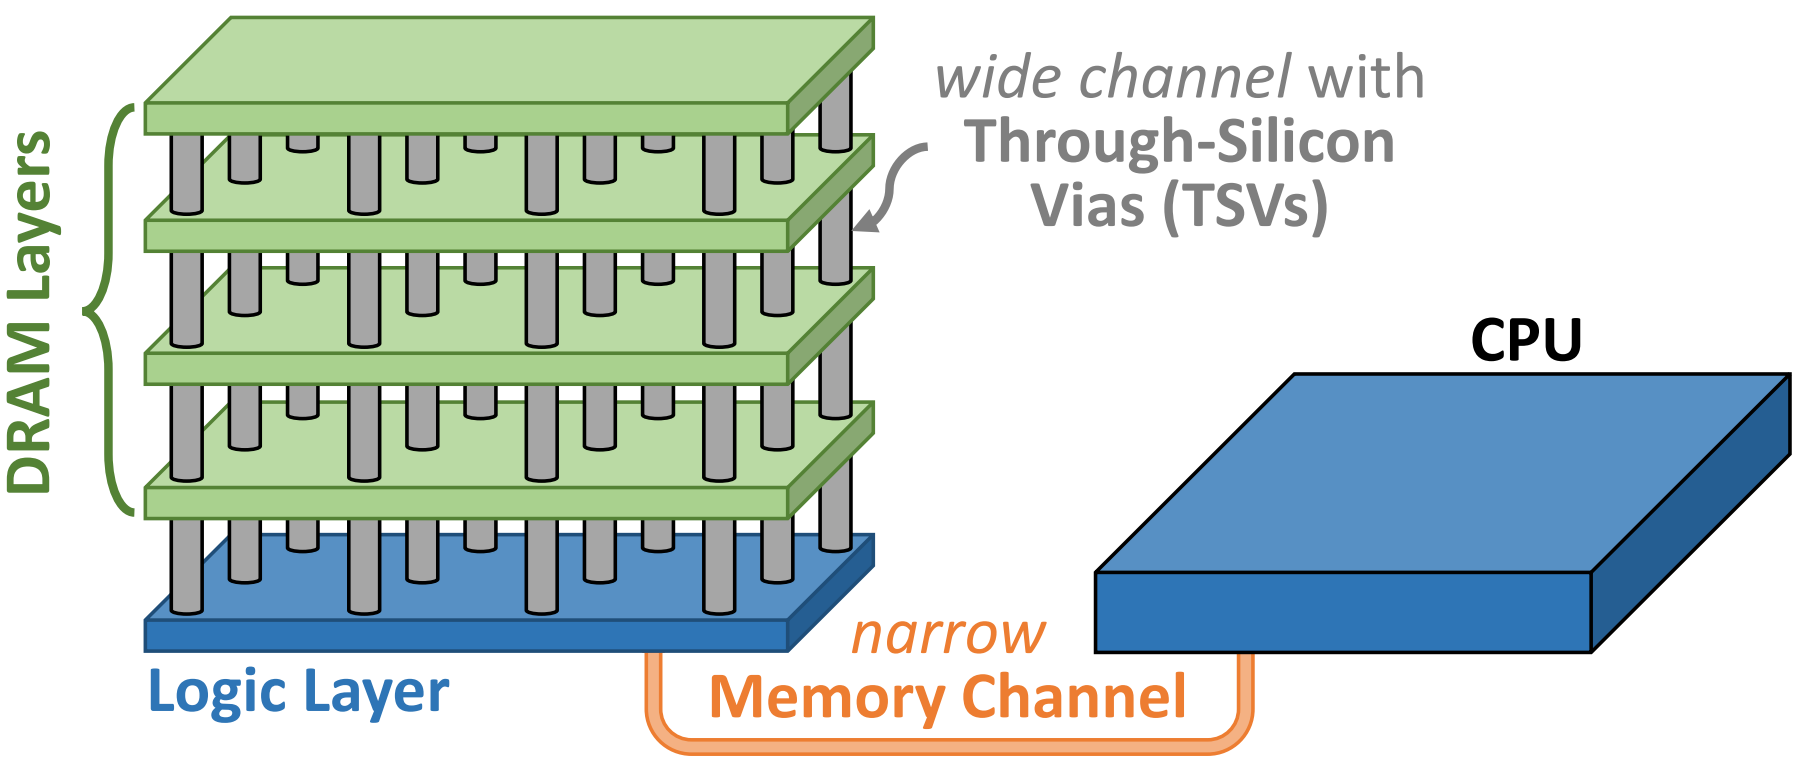
\includegraphics[width=0.9\textwidth]{figures/3DStack.png}
    \caption{3D堆叠内存结构}
	\label{3DStack}
\end{figure}

与此同时由于人工智能(Artificial Intelligence,AI)的兴起,许多专用于神经网络的PIM加速芯片也被设计出来,其中较为著名的就是三星的HBM-PIM(High Bandwidth Memory,HBM)产品\cite{SamsungHBMPIM},该产品采用20nmDRAM工艺,使用3D堆叠技术堆叠封装了4层裸芯(Die),每层die的bank组内增加了专门用于做16位浮点数乘加操作的PIM单元以处理神经网络中的矩阵操作。此外三星的另一个产品AxDIMM\cite{AxDIMM}也采用了近存计算的技术,其将DRAM芯片(Chip)和一块FPGA处理单元整合到一块有着DDR4标准接口的主板上,主要用于加速推荐模型(Recommendation Model)的向量嵌入查找任务(Embedding Lookup)。海力士也提出过存内加速器AiM\cite{AiM}用于加速AI,与三星的HBM PIM不同的是,AiM基于GDDR6(Graphics Double Data Rate V6)内存,为每个bank装配PIM单元,通过设计互连总线和全局缓存实现各个PIM单元的高效互连。近些年国内的公司阿里巴巴推出过近存计算产品\cite{AlibabaPIM},同样采用的是3D堆叠技术将逻辑die和数据die堆叠封装在一起,通过TSV高速传输数据。逻辑die上分别设计了用于向量排序和矩阵乘法的计算单元处理不同类型的任务。

\subsection{近存硬件UPMEM}
然而上述工作因为各种复杂的原因难以落地使用和量产,甚至大部分基于模拟器,使得PIM技术的推广与使用犹如空中楼阁。近几年,一款号称真正可商用的PIM硬件横空出世:UPMEM作为第一款可以商用的近存计算处理器产品\cite{UPMEMHotChips},有着更加通用的处理能力、高速的内存带宽、低廉的接入成本以及完备的开发生态。UPMEM本身是一条2400MHz的有着标准DDR4内存接口的内存插块(Dual In-line Memory Module,DIMM),可以像正常的内存条一样插在Intel CPU的服务器上。每个双核服务器最多可以插入20条UPMEM(需要为每个CPU留出空余的DIMM插口插入普通的DDR4内存)。如\ref{UPMEMArch}所示,一个UPMEM内存条上有2个rank,每个rank拥有8个chip,每个chip中包含着8个bank,每个DPU独占其中一个内存bank。因此一台服务器能够拥有2560个DPU并行处理任务。

\begin{figure}[!htbp]
	\centering
    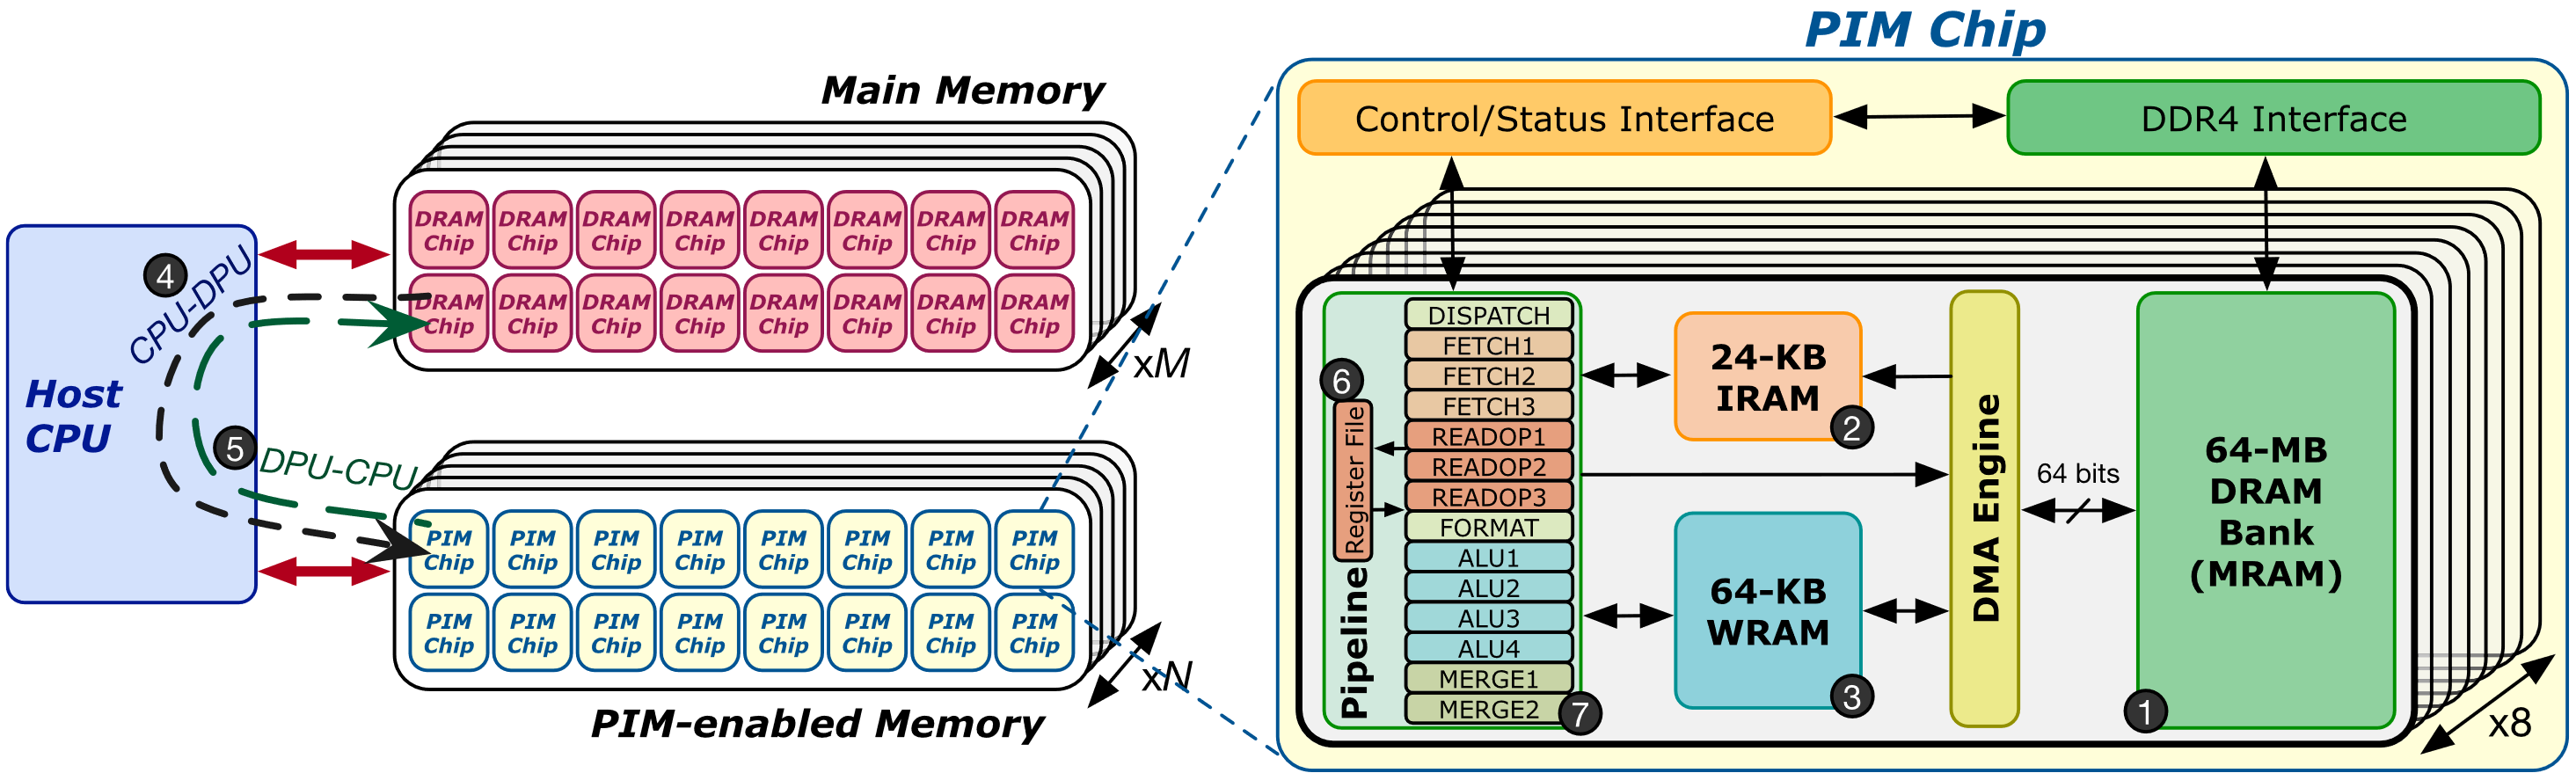
\includegraphics[width=0.9\textwidth]{figures/UPMEMArch.png}
    \caption{UPMEM微架构,图左为UPMEM内存和主机CPU的交互,图右为UPMEM芯片内部组件}
	\label{UPMEMArch}
\end{figure}

每个DPU拥有一个标量顺序(Scalar In-order)多线程的RISC核心,拥有24个物理线程和一个精调的(fine-grained)14级流水线。其中为了避免实现复杂的数据转发和流水线互锁电路 \cite{UPMEMHotChips},同一线程内的两个连续指令必须间隔 11 个周期才能被调度(只有最后三级ALU4、MERGE1、MERGE2可以和下一条指令的 DISPATCH、FFTCH 阶段并行执行)。因此至少同时有11个线程同时运行才能最大程度利用流水线。同时每个DPU的每个线程都有24个可用的32bit的寄存器,需要分奇偶访问。

UPMEM采取哈佛架构,将数据和指令分别存放,拥有24KB的指令存储器IRAM(能存放4096条48位指令)和64KB的数据存储器WRAM。DPU在工作时会在取指阶段访问IRAM,在访存和执行算术运算时访问WRAM。此外还存在存储层级MRAM,其就是每个DPU独占达的DRAM Bank,用于存放和CPU进行通信的数据,拥有较大的存储空间(64MB)。WRAM和MRAM除了在存储容量上的不同之外,由于WRAM本身属于静态RAM(Static Random Access Memory,SRAM),而MRAM就是正常的动态RAM(Dynamic Random Access Memory,DRAM),二者的访问速度存在着数量级的差别。再加上DPU无法直接访问MRAM需要通过WRAM进行中转,因此常规的访问方式是经过内置的DMA引擎将程序用到的大批量的数据从MRAM传输到WRAM中,再在WRAM中去频繁访存和计算。可以将WRAM视作通常意义上的Cache,而MRAM则类似于普通内存,不同之处在于WRAM对开发人员不透明,需要手动管理。

UPMEM在硬件的基础上开发了一套完整的软件栈和工具链方便开发人员在其上搭建应用,包括DPU程序的运行时库、编译器,以及主机端调用DPU程序的API库,以及功能强大的调试器dpu-lldb。UPMEM的编程模式为单程序多数据(Single Program Multiple Data,SPMD)模型,DPU及其独占的bank相对于CPU来说类似于一个协处理器,CPU端被称为host端,而DPU端被称为device端。由CPU主动地将编译好的DPU程序装载入DPU并准备数据传输到DPU,再启动DPU执行程序,执行结束后收集结果或执行下一轮的任务。CPU和DPU之间的通信需要使用UPMEM提供的主机端API库,而DPU和DPU之间无法直接通信需要到CPU搬移到内存中进行中转。

有许多工作对UPMEM的硬件特征做了系统且全面的测试\cite{BenchmarkingMutlu,BenchmarkingGermany,BenchmarkingUBC,BenchmarkingUPMEM,uPimulator},其中,Gómez-Luna等人\cite{BenchmarkingMutlu}的测试工作较为全面且权威。在这些评测中,不难发现UPMEM的硬件优势主要有下面几点:
\begin{itemize}
	\item [1)] 
	高存储容量和传输带宽,忽略WRAM等高速缓存,MRAM本身有64MB,2560个DPU共有160GB内存,远超市面上常用显卡的显存,每个MRAM的传输带宽大约为700MB/s,当2560个DPU并行工作其聚合带宽能够达到1.7TB/s,WRAM的聚合带宽更是能够达到6.8PB/s。      
	\item [2)]
	高并发和细粒度并发控制,如上所述,2560个DPU可以同时工作,每个DPU内部还可以控制24个线程进行更加细粒度的控制,虽然大多数测试中在跑常规测试集(Benchmark)时,超过11个线程并发就会让核心达到饱和,按照这个方式计算,整个PIM系统的并发线程数量能够达到近3w。
	\item [3)]
	高能效比,PIM设备由于减少了数据的多层级搬移可以大大降低能耗,文章\cite{BenchmarkingMutlu}中测试,UPMEM的能效比高于运行同等任务且优化成熟的CPU和GPU。
\end{itemize}

虽然UPMEM有上述的许多优点,作为商用近存计算硬件能够充分支持并行计算,但同时UPMEM的局限性也十分明显:
\begin{itemize}
	\item [1)] 
	UPMEM由于硬件资源十分有限,只支持32bit的整数加减法和8bit的乘法,其他的算术操作包括64bit的相关操作,乘除操作,浮点操作都是使用软件实现,效率较为低下;同时UPMEM本身主频不高,DPU处理器的规模受限,即使是32bit加法的MRAM计算访存比也只有1:4\cite{BenchmarkingMutlu},这些充分说明UPMEM的计算能力弱,更加适合内存瓶颈的任务。
	\item [2)]
	UPMEM的通信效率低,host和device的传输效率本身不高,只有大批量传输连续数据时才能勉强达到DDR4内存的传输带宽,同时DPU直接彼此独立缺乏有效的通信手段,只能通过CPU主动中转数据,效率更加低下。因此UPMEM不适合那些需要多核频繁通信的任务。\cite{BenchmarkingMutlu}。
\end{itemize}

\subsection{UPMEM相关应用}
自UPMEM可商用以来,有许多研究者就此硬件做出了许多工作。其中较为基础的一类是针对UPMEM硬件特征构建软件栈或对硬件做修改。如Khan等人\cite{CINMCompiler}针对包括UPMEM在内的诸多近存计算硬件构建了编译器,以支持开发人员在更高的抽象层级编程。同样的,Chen等人\cite{SimplePIM}也针对UPMEM硬件抽象更为高级的软件栈,包括对DPU的元数据管理、主从通信以及批处理模式三个大主要模块。同时,还有部分工作专注于拓展UPMEM基础软件库。Giannoula等人\cite{SparseP}开发了基于UPMEM的稀疏矩阵向量乘法(Sparse Matrix Vector Multiplication,SpMV)库,支持多种稀疏格式的矩阵以及数据格式,设计了多种数据映射和优化方法以适应不同的场景。Item等人\cite{TransPimLib}在UPMEM上开发了一套基于查找表(Look UP Table,LUT)和CORDIC (coordinate rotation digital computer)迭代的超越函数库,以一定的精度范围内支持了包括三角函数、指数对数、双曲线、平方根等复杂计算。Noh等人\cite{PID-Comm}针对UPMEM的DPU之间通信慢的问题,开发了一套支持多种通信模式的高效通信框架。除此之外,有部分工作在了解了UPMEM硬件的优缺点后,试图对UPMEM的硬件本身进行修改。北大的Zhou等人\cite{DIMM-Link}为解决UPMEM的通信慢的问题,增设外部数据连接电路联通物理相邻的DIMM,并设计数据转发和传输算法提高数据传输效率。

另外一大类重要的工作专注于利用现有UPMEM硬件去加速不同领域的应用,主要涉及到生物基因、数据库以及人工智能领域。生物基因领域主要是使用UPMEM加速基因测序和基因比对工作\cite{DNAMapping,VariantCalling,RNA-seq,UpPipe,GAPiM},这类工作的本质是字符串匹配为内存瓶颈任务,因此适合使用UPMEM硬件进行加速。数据库领域有许多工作对UPMEM关注密切。比如早期的工作\cite{Skyline}将skyline算子卸载到UPMEM。清华的Kang等人做了一系列的工作\cite{PIM-Model,PIM-Tree,PIM-Trie}将数据库常见的索引如跳表、前缀树的查询卸载到了UPMEM上,并充分设计了负载均衡算法保证查询速度。一些工作\cite{PIM-DB,PIM-Scan}将数据库最基本的查询算子,全部或部分卸载到了UPMEM上。Baumstark等人\cite{PIM—QueryCompile}将查询计划的优化也卸载到了UPMEM上。Lim等人\cite{PIM-Join}将数据库中的连接查询(Join)卸载到UPMEM上,通过巧妙地移位和排序解决了UPMEM因内存交错(Bank Interleave)带来的数据传输性能损失。

UPMEM的高并行和细粒度控制特性使得其非常适合用于AI和神经网络的场景。有相当一部分工作使用UPMEM加速神经网络的推理。Zarif等人\cite{UPMEMEmbeddingLookups}将UPMEM用于嵌入查找(Embedding Lookup)任务的卸载,对于目前较大的嵌入表(Embedding Table)加速效果尤为明显。Gómez-Luna等人\cite{UPMEMTraditionalML}以简单直接的方式卸载了传统机器学习中的基础模型到UPMEM上,包括线性回归、逻辑回归、决策树、K均值聚类,并做了全面丰富的测试,但是测试结果无一表明这些模型的推理都遭受了严重的计算性能瓶颈。Das等人\cite{UPMEMCNN}在UPMEM上分别卸载了嵌入二值神经网络(Embedded Binary Neural Network ,eBNN)和YOLOv3(主要是卸载卷积操作),其主要思想是将卷积神经网络(Convolutional Neural Network,CNN)的权重量化到低bit位,再通过查找表查询低bit浮点数乘积,以消除浮点乘法运算,但这会严重降低模型的精度。Giannoula等人\cite{UPMEMGNN}将图神经网络(Graph Neural Network,GNN)的推理卸载到了UPMEM上,测试结果表明对于稀疏图和较为内存瓶颈的场景中,UPMEM的推理效率提升非常大。最与本课题应用场景相近的工作PIM-DL\cite{PIM-DL}使用UPMEM推理Bert,其通过将矩阵乘法转换为最近邻查找和向量加法,减少了对乘法的需求,从而提高了计算效率。但其最近邻查找是在CPU上完成的,而UPMEM只执行向量加法操作,并没将计算重担完全卸载到UPMEM上。最近也开始有研究者尝试使用UPMEM加速神经网络的训练过程。Gogineni等人\cite{SwiftRL}提出SwiftRL以解决强化学习(Reinforce Learning,RL)中的内存瓶颈问题,将Tabular Q-learning和SARSA(State-Action-Reward-State-Action)等强化学习算法在UPMEM上实现,并适应不同应用场景。Rhyner等人\cite{PIM-Opt}希望在UPMEM实现分布式随机梯度下降算法(Stochastic Gradient Descent,SGD)探究UPMEM的AI训练能力和硬件特点。上述两个训练工作的结果都表明只有在内存瓶颈的应用场景下,UPMEM的训练性能提升较大,而且由于训练过程中存在跨节点通信,扩展性较差无法随数据规模线性扩展。

\section{本章小结}
本章详细地对大模型推理加速的相关技术和论文做了详尽的介绍,从大模型的发展历程和模型结构的分析,了解大模型的推理成本很高,明白了加速推理的关键因素在于解决内存瓶颈或者提升基本算子的性能。随后介绍了模型量化的基本原理,以及用于加速大模型以缓解内存瓶颈的相关工作。然后对大模型推理阶段的基本算子矩阵向量乘做了基本的介绍,并阐述了相关的优化方法。

随后主要介绍了近存计算研究现状。首先梳理的近存计算的历史,包括近存计算的产生原因、发展和现状,一并介绍了其中具有代表性的工作。然后着重介绍了号称第一款可商用的近存计算的硬件UPMEM,包括其硬件微架构和软件栈,同时结合相关测评工作说明了改硬件的基本特性。最后详细地介绍了基于UPMEM硬件上做的相关科研工作,涉及生物基因、数据库和机器学习等诸多领域,对研究现状有了充分的认识。
\chapter{基于近存计算硬件的矩阵向量乘软件优化}
基于在第二章介绍的GEMV的通用两种方法,直接使用float32数据格式进行GEMV的计算的性能非常差,原因是UPMEM硬件不支持浮点数的算术运算而使用软件模拟,其性能大约是int32数据类型格式的算术吞吐的十分之一\cite{BenchmarkingMutlu},因此需要考虑量化。在上一章提到,浮点量化格式往往优于定点量化\cite{ZeroQuantFP};同时测试表明UPMEM的访存较计算更快,计算访存比仅有1:4\cite{BenchmarkingMutlu},因此非常适合用访存换计算。基于上面的两点我们使用基于FP8数据格式\cite{FP8}的查找表算法。量化的大致思路是使用机器学习的方式以少量的校准数据集调整权重参数以适应基于LUT的GEMV内核。针对反向传播中LUT不可导的问题,可以使用直通估计器(Straight-Through Estimator,STE)解决\cite{NonuniformQuant}(STE简单来说就是跳过LUT自身的梯度下降,将误差直通传递到上一层,通过调整上一层的矩阵权重来实现误差最小化,这是一种非均匀量化的手段)。受篇幅限制,本文将不讨论具体的量化方法而专注于设计通用的矩阵向量乘内核。此外为了和Llama2-7B保持一致,没有特别说明,本章中涉及到的权重矩阵的维度皆为$4096\times 4096$,同时本章所有讨论的优化都是建立在单个DPU的推理优化。因此单个DPU的GEMV内核的正常输入为4096维度FP8数据格式的激活向量,4096维度FP8数据格式的权重方阵,最终计算得到的结果为4096维度的结果向量。

本章将基于量化后FP8数据格式的查找表算法优化GEMV算子,主要分两个层次进行优化,首先优化WRAM的数据局部性,减少MRAM访存;其次优化寄存器的数据局部性,减少WRAM的访存。

\section{基于多级存储的查找表分块算法}
UPMEM的MRAM访问是通过DMA引擎,速度较慢,并且只在大批量数据传输时带宽较高,针对该硬件特性,本节针对存储层级MRAM做访存优化,提高WRAM的数据局部性。

\subsection{矩阵向量乘查找表基础}
查找表(Look Up Table,LUT)是非常典型的存储换计算的技巧,常常被用在某些边端设备或者计算能力有限的硬件上以支持复杂计算。由于UPMEM硬件本身较弱的计算能力,以及较低的计算访存比,非常适合使用访存换计算的方法。一般意义上的查找表就是对于函数$f(x_1,x_2,\cdots,x_n)=y$,在一定的定义域范围和精度内穷举所有自变量的组合,并提前计算得到每种组合对应的函数值,制作成一张映射表,此后的函数计算无需计算而只需查表即可。由于计算机只能离散有限地表示数值,每种特定位宽的数是天然可穷举的,例如对于$n bit$的数作为自变量,其本身有$2^n$种不同的数值,两个$n bit$的数作为自变量,则有$2^{2n}$个不同的组合。

\begin{figure}[!htbp]
	\centering
    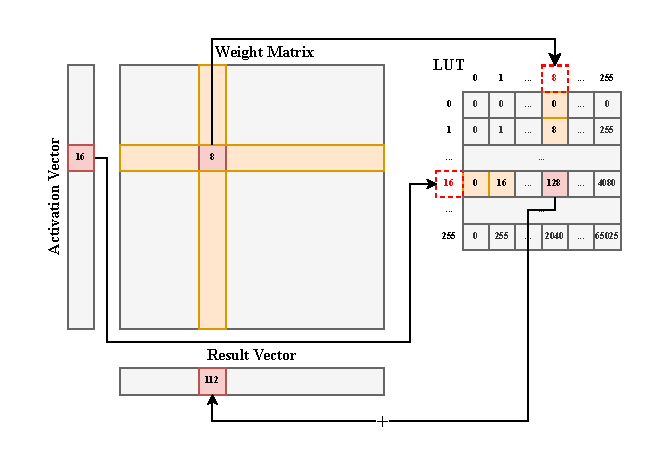
\includegraphics[width=0.9\textwidth]{figures/LUT.pdf}
	\caption{基于查找表的矩阵向量乘}
    \label{LUT}
\end{figure}

这里举例GEMV的8bit乘法查找表的设计,如图\ref{LUT}所示,其中有一张数据类型为uint8的乘法查找表(为了直观采用uint8数据格式)。由于两个操作数都为8bit,因此输入一共有$256\times 256=2^{16}$种组合,因此可以提前构建一个256行256列二维数组存储查找表LUT,第一个操作数的数值代表行索引,第二个操作数的数值代表列索引,行索引和列索引交叉索引到的元素值为两个操作数的乘积。例如在进行GEMV运算时,要计算激活向量(Activation Vector)中某个值为16的元素和权重矩阵中某个值为8的元素的乘积,现只需要访问提前构建好的二维数组(查找表)的第16行第8列的元素即可,得到答案为128,再加到结果向量(Result Vector)的对应位置上。当然这里加法计算同样可以通过构建一张8bit的加法查找表消除。这样,8位宽下任意数据格式的任意二元算术运算都可以按照上述的查表方式将计算转换为访存。同时上述访存过程仅仅涉及最简单的数组索引计算,几乎能够得到所有硬件的支持,从而降低了对硬件算术能力的要求。

上述乘法查找表的构建存在冗余,因为乘法满足交换律,因此上述$256\times 256$的矩阵只需要保存上三角或下三角即可。甚至能够进一步将8bit的乘法拆成多步4bit的乘法、加法和移位操作,但这两种做法无疑都会增加计算复杂度,对于在UPMEM上需要频繁访问的查找表而言是不合适的。同时查找表能够按照行划分成为子表,例如上述uint8的乘法查找表,当能够确定某个操作数的变化范围在[0,64)时,只需要上述查找表的前64行即可满足计算,即每一行和多行的组合都是属于8bit乘法查找表的子查找表,当空间受限时,可以按需载入子查找表。在此我们特别约定:1)查找表的大小和构建方式都如上述所描述,n bit的二元运算查找表表项为$2^{2n}$;2)二元运算查找表通过两个索引(分别是行列索引)确定查找值,约定这里的索引在后文称作索引值(row/col index),查表得到的值为元素值(element);3)后文如果没有特别说明,子查找表指的是原查找表二维数组的不同行的组合,即确定行索引值的范围的子表。

\subsection{分块载入查找表卸载乘法}
直接使用8bit乘法查找表的方法在UPMEM中卸载GEMV计算存在诸多问题,首当其冲的就是WRAM的空间限制:由于查找表在执行GEMV运算时需要频繁访问,因此必须要将其载入WRAM高速内存中才会有较好的性能。然而8bit的查找表光是表项就有$256x256=2^{16}=64K$项,如果按照表中每个元素刚好占用1字节,则查找表需要占用空间64KB,而WRAM的容量只有64KB,除了用户数据之外至少需要为各个线程的堆栈留存一部分空间,因此无法将整个查找表载入WRAM。

解决办法就是分块载入查找表,每次只执行数据范围落在当前载入的子查找表覆盖的范围内的计算。但是此时需要注意的一点就是数据的重用性:权重矩阵无法一次性全部载入WRAM,从MRAM载入WRAM的带宽远低于WRAM与核心交互的带宽,分多次载入子查找表后需要避免因为计算不完整而重复载入矩阵。基于上述考虑,我们设计了基于分块载入查找表卸载GEMV中的乘法的算法,具体如图\ref{LUTBlock}所示,激活向量(Activation Vector)和结果向量(Result Vector)完整载入WRAM中,将查找表拆分成16个子查找表,行索引范围被划分为在$[0-15),[16-31),\cdots,[240,256)$16个区间。

\begin{figure}[!htbp]
	\centering
    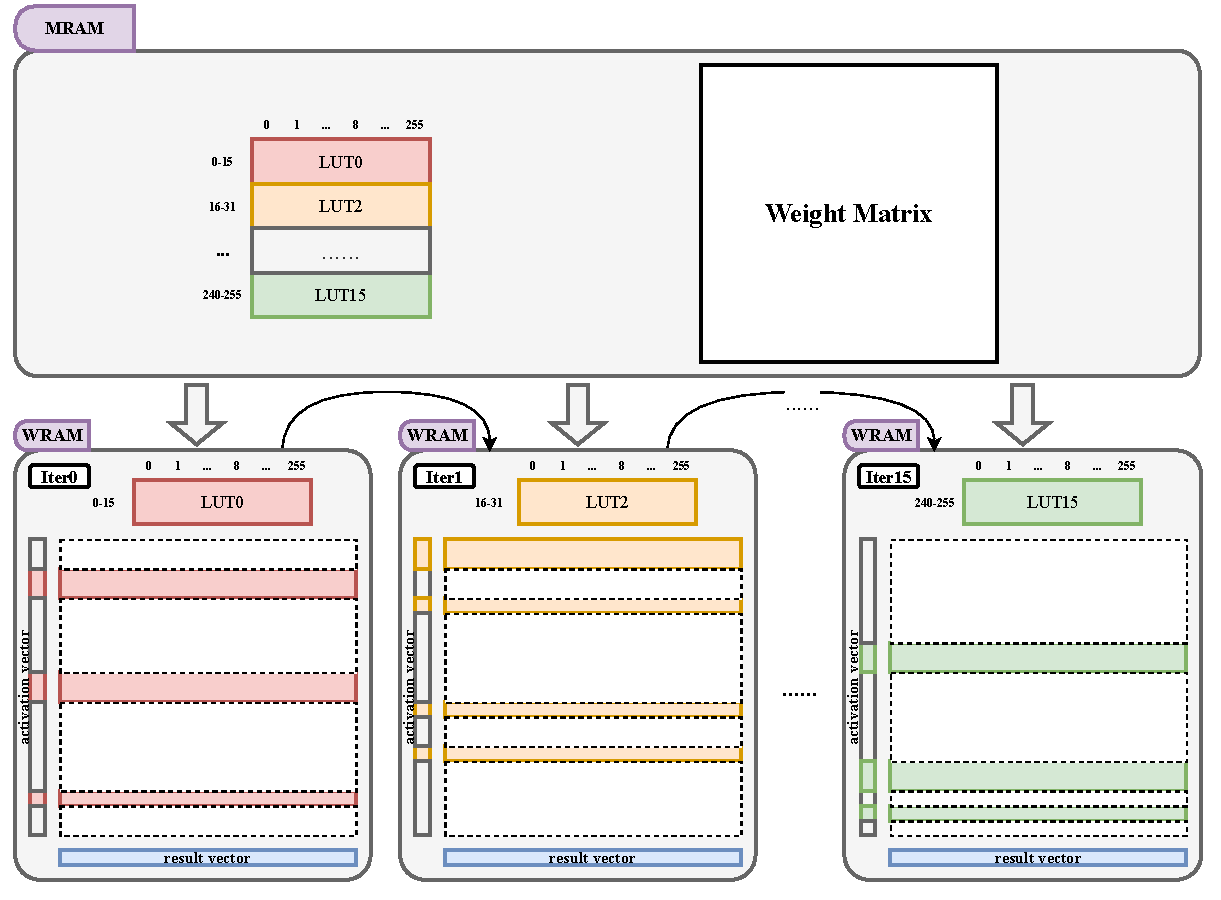
\includegraphics[width=0.9\textwidth]{figures/LUTBlock.pdf}
	\caption{分块载入查找表卸载GEMV中的乘法}
    \label{LUTBlock}
\end{figure}

该算法需要进行子查找表个数次迭代,每次迭代流程大致为:将子查找表载入WRAM中,遍历激活向量,对于每个元素判断其值是否在当前子查找表的行索引值区间内,对于满足要求的元素,将该元素所对应的权重矩阵(Weight Matrix)的行向量从MRAM载入WRAM,执行查表乘法计算并加到结果向量上;对于不满足要求的元素直接跳过,等待下一次迭代再进行判断。如此一来完全没有将数据重复地从MRAM搬移到WRAM中,无论是查找表还是权重矩阵,都只从MRAM中搬移到WRAM中一次,实现了非常良好的WRAM数据局部性。

\subsection{基于数制映射表卸载加法}
想要完整卸载GEMV算子的所有计算仅仅使用上述分块查找表卸载乘法远远不够,上述方法虽然使用分块载入的方式解决空间上的限制,但是在计算加法时无法简单套用类似的思路:由于使用的数制是FP8,硬件加法无法支持,同时由于累加的操作特性,FP8加法的所在查找表区间是动态变化的,无法事先静态地确定并载入子查找表,直接从MRAM中读取性能就会非常差。一种方式是直接使用软件模拟:FP8常用的有两种格式\cite{FP8},如表\ref{FP8Format}所示,我们选用E4M3格式的FP8进行推理,因其相较于E5M2具有更高的精度(E5M2相较于E4M3拥有更高的动态范围更适合训练)。其数据格式并不完全符合IEEE754,取消了无穷的表示缩减了NaN的表示范围以容纳更多规格化数,其他部分均符合IEEE754的标准。
    
\begin{table}[!htbp]
    \caption{FP8常用两种格式二进制细节}
    \label{FP8Format}
    \begin{tabular}{lll}
        \toprule
        & E4M3 & E5M2 \\ 
        \midrule
        Exponent bias & 7 & 15 \\
        Infinities & N/A & S.11111.00\textsubscript{2} \\
        NaN & S.11111.11\textsubscript{2} & S.11111.\{01, 10, 11\}\textsubscript{2} \\
        Zeros & S.0000.00\textsubscript{2} & S.00000.00\textsubscript{2} \\
        Max normal & S.1111.10\textsubscript{2} = 1.75 * 2\textsuperscript{8} = 448 & S.11110.11\textsubscript{2} = 1.75 * 2\textsuperscript{15} = 57,344 \\
        Min normal & S.0001.00\textsubscript{2} = 2\textsuperscript{-6} & S.000001.00\textsubscript{2} = 2\textsuperscript{-14} \\
        Max subnormal & S.0000.11\textsubscript{2} = 0.875 * 2\textsuperscript{-6} & S.000000.11\textsubscript{2} = 0.75 * 2\textsuperscript{-14} \\
        Min subnormal & S.0000.01\textsubscript{2} = 2\textsuperscript{-9} & S.000000.01\textsubscript{2} = 2\textsuperscript{-16} \\ 
        \bottomrule
    \end{tabular}
\end{table}

如果直接使用软件模拟,计算两个浮点数的流程的大致为:对阶、尾数求和、规格化、舍入、溢出处理,虽然不用处理无穷等特殊情况,但是上述几个步骤中涉及到大量的移位操作和逻辑操作,由于UPMEM的一个周期至多只能执行一条指令\cite{UPMEMHotChips},因此这些位运算和逻辑运算指令开销不能忽视,而且由于规格和非规格数的区别存在大量的条件判断和跳转语句,同样非常影响性能。

分析量化大模型的推理流程,以W8A8的量化为例,在进行线性层推理时,会先将8bit量化的权重和激活解量化到16bit,再调用矩阵乘法库中的16bit矩阵向量乘算子,得到16bit的结果,再转换回8bit的结果向量传递给下一个算子。受此启发,
可以将E4M3格式的FP8展开成int32,使用int32进行加法计算和中间结果的保存(硬件不支持int32乘法但是支持加法),在得到最终的结果向量后再转回FP8数制以便后续的传输。具体的展开形式可以很简单,E4M3的符号位不变置于int32的符号位,同时根据指数位置判断该数是否为规格化数,若是规格化数,则需要将尾数的低三位前面添1形成4位尾数;若不是规格化数,则正常取尾数。然后假设指数部分的值为e,将尾数左移$max(e-1,0)$位即可。如图\ref{LUTBS}所示,FP8数0 0010 110转为int32为0...11100,FP8数0 0000 110转为int32为0...110,二者相加得0...100010,这个时候反转回FP8应该首先判断是否为规格数,显然该数为规格化数,需要将int32数右移直至前导第一个1到最低第4位上(计算舍入)即可。

但其实同样可以使用一张数制映射表代替上述复杂的逻辑操作,如图\ref{LUTBS}中的MapLUT,是一个表项为256的一元映射查找表,提前将FP8展开存储在该张映射表中,在计算时展开操作就可以换为查表操作。更进一步,原本的乘法查找表元素为单字节FP8,现在将其替换为其对int32的映射项,变为四字节。这样查询出来的乘积就是int32的展开格式,直接加到同样每个元素扩展为32位的结果向量中。最后,基于查找表MapLUT再通过二分查找将结果向量中的每个元素还原成FP8以便后续的传输。

\begin{figure}[!htbp]
	\centering
    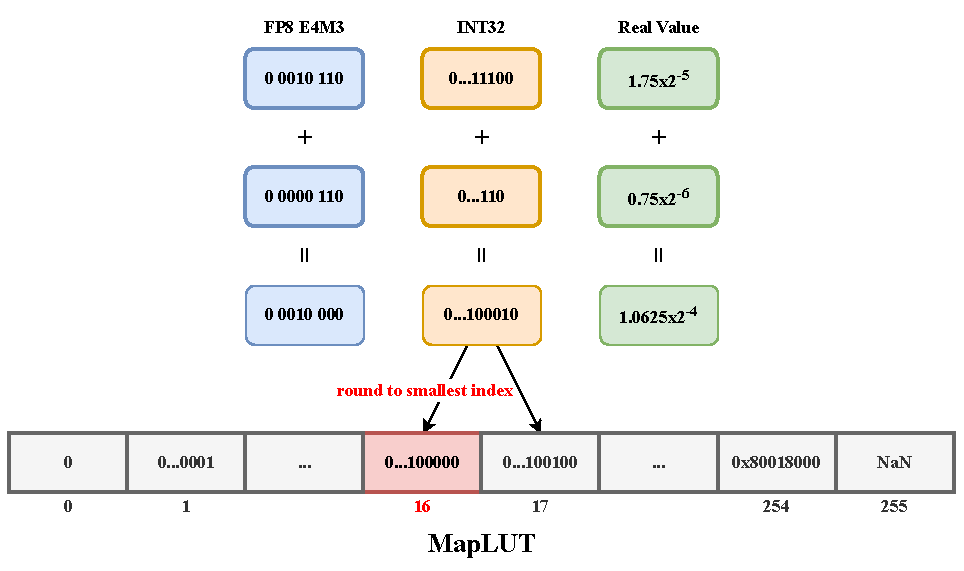
\includegraphics[width=0.9\textwidth]{figures/BinarySearch.pdf}
	\caption{数制映射表卸载GEMV中的加法}
    \label{LUTBS}
\end{figure}

在查找的过程中,可能会遇到舍入问题,即计算出来的元素值无法精准匹配查找表中的元素,其原因是使用int32进行加法运算时保留了相当的精度没有舍入,这个时候会出现待查找的值处于查找表两个相邻元素值之间,如图\ref{LUTBS}所示,为了简化计算加速查找我们直接选择索引值较小的那个数作为查找结果:一方面转为int32进行中间结果的加法运算相对于直接使用FP8计算保留了相当大精度,这里只是将最终结果进行转换因此精度损失整体来讲不大;另一方面精度损失仍然可以通过离线的基于机器学习的量化工作优化消除。这种舍入方式我们这里称之为向最小索引值舍入(Round to Smallest Index),这种舍入其实本质和IEEE754标准的向零舍入(Round toward Zero)是同一种舍入规则。

\subsection{算法小结}

\begin{algorithm}[!htbp]
    \caption{基于多级存储的查找表分块算法(LUT-M)}
    \label{LUT-M}
    \begin{algorithmic}[1]
        \Require $Vector[M], Matrix[M][N], LUT[256][256], MapLUT[256]$; % input
        \Ensure $Result\_8[N]$; % output

        \State $\textbf{define}\; SubLUT[16][256],\;MatRow[N],\;Result\_32[N]$

        \For{$i \gets 0$ \textbf{to} $15$}
            \State $\textbf{mram\_read}(SubLUT, LUT[16i \cdots 16i + 15], 16K)$
            \Comment{\textcolor{blue}{parallel read}}
            \For{$j \gets 0$ \textbf{to} $M - 1$}
                \If{$Vector[j] \;\textbf{not in}\; [16i, 16i+15]$}
                    \State \textbf{continue}
                \EndIf
                \State $\textbf{mram\_read}(MatRow, Matrix[j], N)$
                \Comment{\textcolor{blue}{parallel in N for each tasklet}}
                
                \For{$k \gets 0$ \textbf{to} $N-1$}
                \Comment{\textcolor{blue}{parallel in N for each tasklet}}
                    \State $Result[k] \gets Result[k] + SubLUT[Vector[j] \& \text{0xF}][MatRow[k]]$
                \EndFor
            \EndFor
        \EndFor

        % 调用二分查找函数
        \State $Result\_8 \gets \textbf{BinarySearch}(Result\_32, MapLUT)$
        \Comment{\textcolor{blue}{parallel in N}}
        \State \Return $Result\_8$
    \end{algorithmic}
\end{algorithm}

至此,可以完全卸载GEMV算子的全部运算到UPMEM上,我们在这里对上述方法进行总结,给出算法如\ref{LUT-M}所示,假设M和N都为4096,那么激活向量大小为4KB,32bit的结果向量的大小为16KB,转成对应的FP8向量需要占用4KB的空间,但是可以直接覆盖写入激活向量以节省空间,将查找表分成16份,每个子查找表的大小为16KB,载入的矩阵一行的大小为4KB,FP8到int32的映射表大小为1KB,总共占用WRAM空间41KB,剩余23KB给各个线程分配堆栈空间完全足够用。在这种设计下,权重矩阵的所有行总共只需要从MRAM中载入WRAM中一次,LUT的每个子表同样也只载入一次,FP8和int32的相互映射也是直接在WRAM中完成,充分提高了数据的重用性。

\section{基于缓存的矩阵行列重排算法}
UPMEM访问WRAM的速度较快,当流水线充满时,且访问带宽不受访问模式影响(顺序、随机),且任何8byte以下的数据访问都只会消耗一个时钟周期\cite{BenchmarkingMutlu}。在上一小节主要针对MRAM的读写做了优化,提高了WRAM的数据局部性,这一小节主要针对WRAM做优化,提高寄存器的数据重用。

\subsection{矩阵行重排}

\begin{figure}[!htbp]
	\centering
    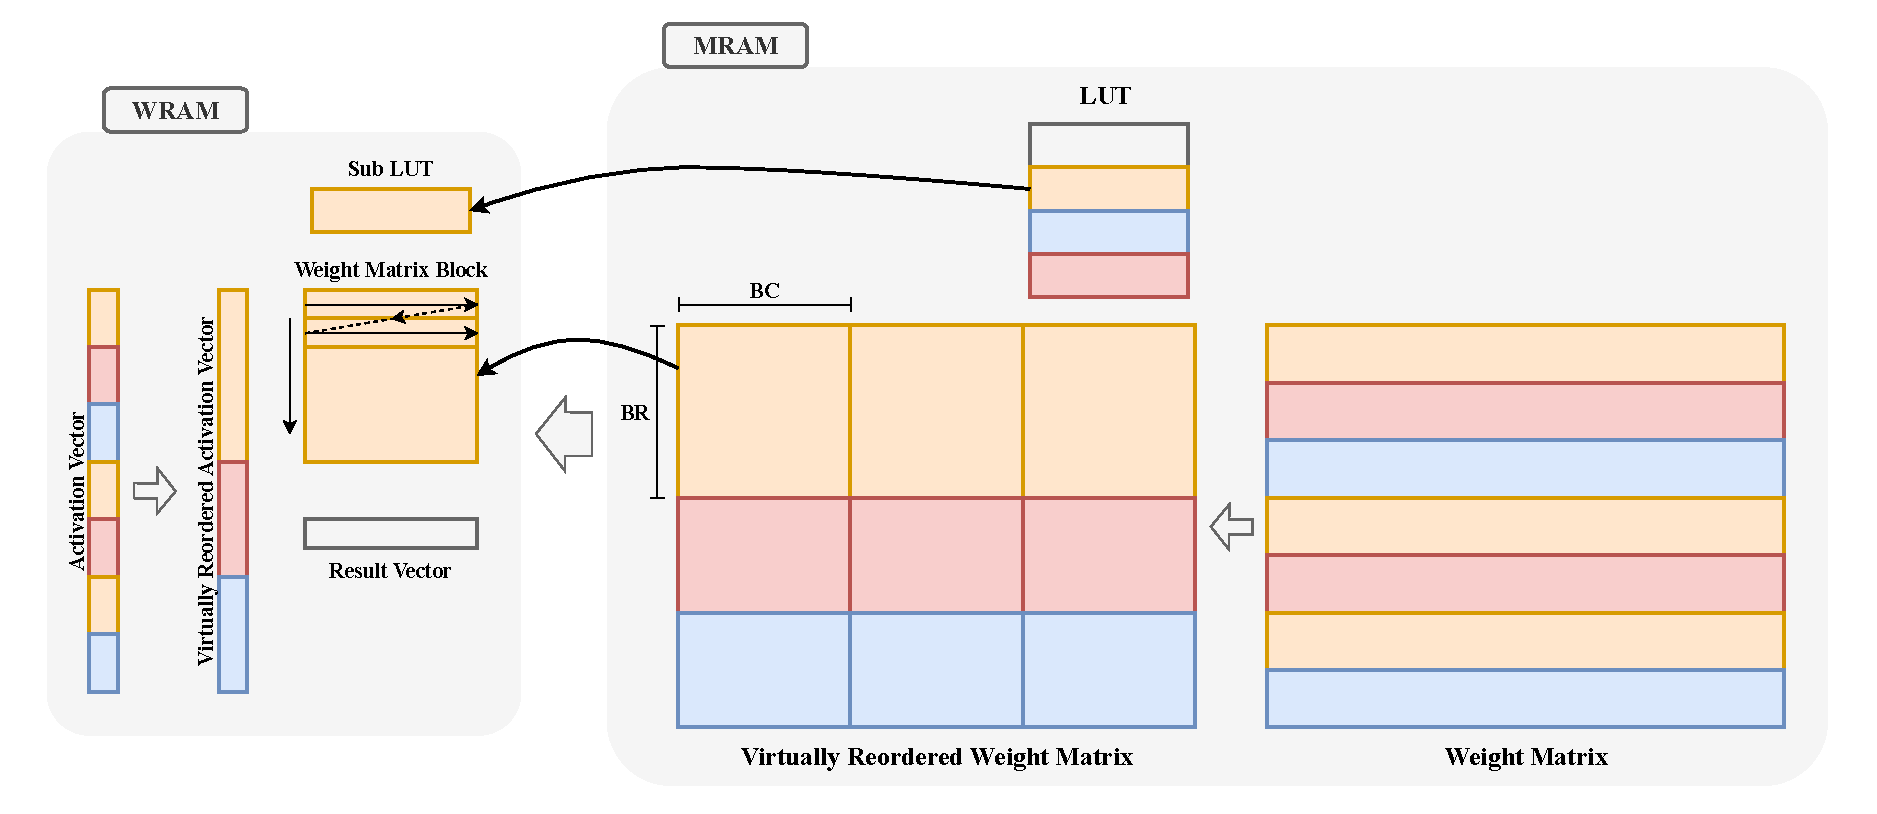
\includegraphics[width=0.9\textwidth]{figures/LUTRow.pdf}
	\caption{矩阵行重排计算示意图}
    \label{LUTRow}
\end{figure}

针对算法\ref{LUT-M},可以观察到每完成权重矩阵的一行计算就要读写各一次结果向量,有很大的开销,这里基于此前提到的算法做出修改如图\ref{LUTRow}所示,此前由于考虑权重矩阵一行的向量会较长无法同时载入多行,在这里可以依据激活向量的值的分布对权重矩阵进行分块,划分成BR(Block Row)行BC(Block Column)列的子矩阵。

\begin{algorithm}[!htbp]
    \caption{行重排的矩阵向量乘算法(LUT-W-R)}
    \label{LUT-W-R}
    \begin{algorithmic}[1]
        \Require $Vector[M], Matrix[M][N], LUT[256][256], MapLUT[256], BR, BC$; % input
        \Ensure $Result\_8[N]$; % output

        \State $\textbf{define}\; SubLUT[16][256],\;SubMat[BR][BC],\;Result\_32[N]$
        
        \For{$i \gets 0$ \textbf{to} $15$}
            \State $\textbf{mram\_read}(SubLUT, LUT[16i \cdots 16i + 15], 16K)$
            \Comment{\textcolor{blue}{parallel read}}

            \State $\textbf{define}\; Offset[BR],\;Index[BR],\;vidx=0$
            \While{$vidx < M$}
                \State $row \gets 0$
                \While{$row < BR$ \textbf{and} $vidx < M$}
                \Comment{\textcolor{blue}{parallel in BR for each tasklet}}
                    \If{$Vector[vidx] \;\textbf{in}\; [16i, 16i+15]$}
                        \State $Index[row] \gets vidx,\;row \gets row + 1$
                        \State $Offset[row-1] \gets SubLUT[Vector[vidx] \& \text{0xF}]$
                    \EndIf
                    \State $vidx \gets vidx + 1$
                \EndWhile
                \For{$j = 0$ \textbf{to} $N - 1$ \textbf{step} $BC$}
                    \For{$k = 0$ \textbf{to} $\text{row} - 1$}
                    \Comment{\textcolor{blue}{parallel in BR for each tasklet}}
                        \State $\textbf{mram\_read}(SubMat[k], \&Matrix[Index[k]][j], BC)$
                    \EndFor
                    \For{$k = j$ \textbf{to} $j + BC - 1$}
                    \Comment{\textcolor{blue}{parallel in BC for each tasklet}}
                        \State $temp \gets Result\_32[k]$
                        \For{$l = 0$ \textbf{to} $row - 1$}
                            \State $temp \gets temp + *(Offset[l] + SubMat[l][k] \times ele\_width)$
                        \EndFor
                        \State $Result\_32[k] \gets temp$
                    \EndFor
                \EndFor
            \EndWhile
        \EndFor

        % 调用二分查找函数
        \State $Result\_8 \gets \textbf{BinarySearch}(Result\_32, MapLUT)$
        \Comment{\textcolor{blue}{parallel in N}}
        \State \Return $Result\_8$
    \end{algorithmic}
\end{algorithm}

对于子矩阵,可以一次性全部载入,进而使用GEMV的内积计算方式,将结果向量某个元素的值缓存在寄存器中,完成了子矩阵的一列计算后再写入内存 。注意这里不改变矩阵的行列主存格式,依然按照行主存,原因是这里不真实地对矩阵的行进行重排,仅仅是在载入时挑选满足需求的子矩阵行,称之为虚拟重排(Virtually Reordered)。因此行之间不一定是连续的,改为列主存的话无法充分利用DMA引擎的大批量连续数据传输带宽高的特性,好在WRAM的访存模式对访存带宽并无影响,这里仍然按照列进行访存和计算,将子矩阵的一列和对应的激活向量进行向量内积操作,结果加到结果向量对应位置中。每次载入子查找表,就以BR行的粒度载入BC列的子矩阵,当该BR行的所有子矩阵完成了计算后,取寻找下一个BR行的子矩阵直至结束激活向量的所有访问。

具体如算法\ref{LUT-W-R}所示,设置M和N都为4096,且一次性载入的子矩阵大小上限为16KB,可以将BR和BC都设置为128,此时新增的数据结构有子矩阵SubMat,占用空间16KB;有Index数组保存行索引,占用256B;有Offset数组用于保存该行查找表的偏移,占用1KB空间,因此一共多占用了近13KB的WRAM的空间,相比于算法\ref{LUT-M}剩余8KB的空间,分配给各个线程的堆栈足够了。在使用行重排之前,每一行矩阵的计算都要读写各一次4096维度的结果向量。而使用了行重排之后,假设每次子矩阵都是128行,那么每128行才会读写各一次4096维度的向量,单就读写结果向量的提升来说,是128倍。当然每次处理矩阵元素时,不仅仅只做读写向量的操作,还包括读取矩阵元素、查表、相加以及其中隐含的算术逻辑操作,实际提升需要进一步测试。

\subsection{矩阵列重排}
同样针对算法\ref{LUT-M},可以观察到,当激活向量中的某个元素和权重矩阵的一行做乘积时,需要频繁地查找子查找表以获取乘积,然而由于矩阵权重的每个元素为8bit,总共只有256种值,对应的乘积也只有256种值,因此理论上最多只需要查询256次LUT,但是实际的计算情况是矩阵一行中的每一个元素都重新去查询LUT,一共查询了4096次。如果将矩阵的一行按照数值排序,相同的连续数值只需要查表一次,这样就能避免重复查询LUT,提高访存效率。

按照此思想,我们提出列重排如图\ref{LUTCol:Construct}所示,为方便展示工作原理,这里以3bit数据位宽和一个16元素的向量为例,对于权重矩阵的每一行,首先我们保留其索引值,按照元素值进行排序,排序后我们构建一个8个元素的桶(数组)对应3bit数据的所有取值情况,对权重矩阵每一行0-7数值出现的次数进行计数,计数完成的这8个桶,我们称之为Delim数组,$Delim[i]$代表的含义就是值为i的元素出现的次数;接下来设置状态转移方程\ref{DelimDP}。

\begin{equation}
    \text{delim}[i] = \begin{cases}
        \text{delim}[i] - 1, & i = 0 \\
        \text{delim}[i] + \text{delim}[i - 1], & i > 0
    \end{cases}
    \label{DelimDP}
\end{equation}

这样更新之后,Delim才被真正称之为分界数组,然后再将排序后的索引构成的Index数组替换为权重矩阵对应的行向量即可。这个时候Delim数组的值就是指示着矩阵元素值发生变化的分界线。使用这样两个数据结构进行GEMV运算,如果确定了激活向量的元素的值V为2后,相当于确定了要查找的子查找表(查找表的某一行),然后读取Delim数组可以知道,Index数组的索引$(0,7]$的元素值都是1,因此可以通过查找LUT确定这个7个数的乘积都为1(uint8查找表),再读取载入的Index数组确定累加到结果向量的索引完成计算。

\begin{figure}[htbp!]
	\centering
	\subfigure[列重排Index和Delim数组构建]{
		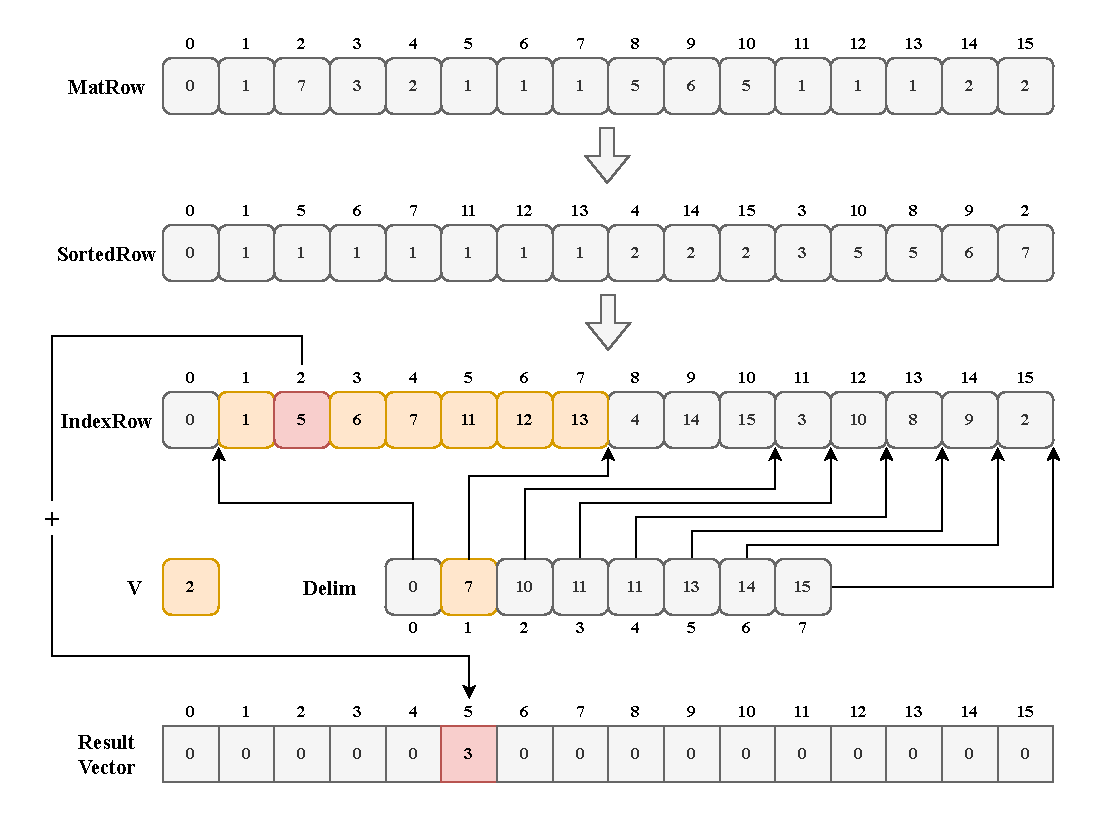
\includegraphics[width=0.5\textwidth]{figures/LUTCol.pdf}
		\label{LUTCol:Construct}}
	\subfigure[列重排并行计算优化]{
		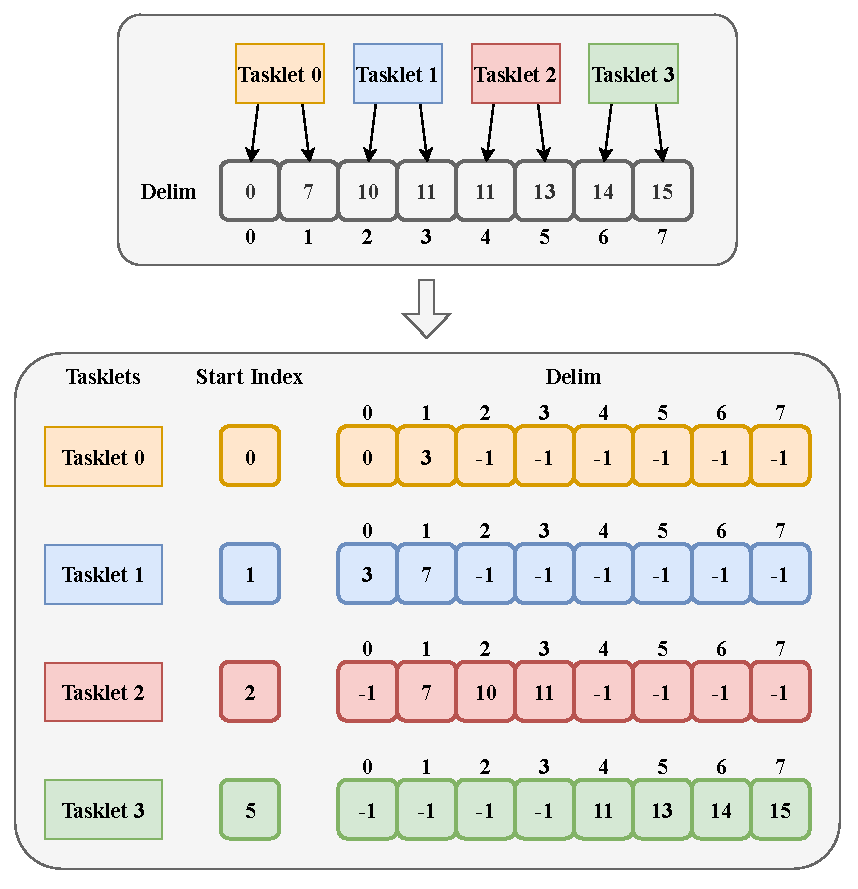
\includegraphics[width=0.4\textwidth]{figures/LUTColParallel.pdf}
        \label{LUTCol:Parallel}}
	\caption{矩阵列重排计算示意图}
    \label{LUTCol}
\end{figure}

但是由于数据的分布情况未知,简单按照Delim长度平均分配给各个线程的任务可能出现严重的负载不均,无法充分利用DPU的并行计算能力。可以看到图\ref{LUTCol:Parallel}中,这16个元素的向量交由4个tasklet进行数据划分执行GEMV,如果按照简单地Delim数组长度平均分,即tasklet0负责Delim数组中索引0和1的计算,tasklet1负责2和3等等,那么就出现负载不均衡:tasklet0负责了8个元素的计算,几乎占据了整个向量计算量的一半,而其他tasklet的计算量非常低,甚至有些只有两个元素的计算量,这些tasklet计算完成后就会被闲置等待tasklet0完成工作。

\begin{algorithm}[!htbp]
    \caption{列重排的矩阵向量乘算法(LUT-W-C)}
    \label{LUT-W-C}
    \begin{algorithmic}[1]
        \Require $Vector[M], DelimMat[M][TN][257], IndexMat[M][N], LUT[256][256], MapLUT[256]$; % input
        \Ensure $Result\_8[N]$; % output

        \State $\textbf{define}\; SubLUT[16][256],\;IndexRow[N],\;Delim[257],\;Result\_32[N]$

        \For{$i \gets 0$ \textbf{to} $15$}
            \State $\textbf{mram\_read}(SubLUT, LUT[16i \cdots 16i + 15], 16K)$
            \Comment{\textcolor{blue}{parallel read}}
            \For{$j \gets 0$ \textbf{to} $M - 1$}
                \If{$Vector[j] \;\textbf{not in}\; [16i, 16i+15]$}
                    \State \textbf{continue}
                \EndIf
                
                \State $\textbf{mram\_read}(IndexRow, IndexMat[j], 2N)$
                \Comment{\textcolor{blue}{parallel read}}
                \State $\textbf{mram\_read}(Delim, DelimMat[j][TaskletId], 514)$

                \State $k \gets Delim[0]$
                \While{$Delim[k] \neq -1$}
                    \State $product \gets SubLUT[Vector[j] \& \text{0xF}][k]$
                    \For{$l \gets (\textbf{if } k=0 \textbf{ then } 0 \textbf{ else } Delim[k-1]+1)$ \textbf{to} $Delim[k]$}
                        \State $Result[IndexRow[l]] \gets Result[IndexRow[l]] + product$
                    \EndFor
                    \State $k \gets k + 1$
                \EndWhile
            \EndFor
        \EndFor

        % 调用二分查找函数
        \State $Result\_8 \gets \textbf{BinarySearch}(Result\_32, MapLUT)$
        \Comment{\textcolor{blue}{parallel in N}}
        \State \Return $Result\_8$
    \end{algorithmic}
\end{algorithm}

回到实际情况,试想一种极端情况:权重矩阵的某一行4096个元素,值全部都是1,这样所有的计算任务都会交由tasklet0执行,其他线程需要等待tasklet0计算完成才能进行下一行的计算,性能会大大降低。因此为了负载均匀,需要重新设计Delim数组的形式:为每个tasklet配备一个Delim数组,然后将任务均分到每个tasklet独享的Delim数组中。

如图\ref{LUTCol:Parallel}所示,将前4个元素的计算分给tasklet0,则tasklet0需要执行一个值为0的计算和三个值为1的计算,那么只需要在Delim数组的0号索引填0,一号索引填3即可,在二号索引填-1表示任务结束不用继续读取Delim数组;tasklet1负责5-8号元素的计算,需要执行四个值为1的计算,只需要在一号索引填7,Start Index处填1表示任务起始的计算值,这样tasklet1就会从1号索引的前一号索引读取起始位置为3+1=4,然后读取4、5、6、7号元素执行计算。其他的tasklet类似。如此以来就能避免负载不均衡的问题。给出对应的算法\ref{LUT-W-C}。

假使M和N都为4096,相比算法\ref{LUT-M},MRAM中多了DelimMat,Matrix变为IndexMat,因为需要记录索引因此矩阵的元素从一字节变为两字节。MRAM仍然足够,当TN(TaskletNum)为16时,WRAM中多了16个Delim数组,大概占用8KB的空间,且MatRow变为IndexRow多占用4KB空间,一共多占用12KB,总共占用WRAM空间53KB,剩余11KB给16个线程分配堆栈空间足够。同时每个tasklet在处理一行矩阵时由原来的4096次查表,变成了现如今最多256次查表,仅仅只是多读取了一个Delim数组,每行矩阵大概由原本的8K WRAM reads变为4.5K WRAM reads,差不多有两倍的性能提升。和此前算法\ref{LUT-W-R}类似,实际过程中查表操作的占比未知,提升需要进一步测试。

\section{本章小结}
本章主要是介绍了在近存计算UPMEM硬件上对GEMV算子的软件优化。首先简要提及了基于查找表的量化手段,介绍了查找表卸载二元算术运算基础。在此基础上提出针对多级存储访存优化的矩阵向量乘算法LUT-M,该算法使用查找表的方法卸载了FP8数据格式的乘法和加法的二元运算,拥有非常好的WRAM数据局部性。随后,更进一步提出了针对缓存访存优化的矩阵向量乘算法,分别对矩阵进行行重排(LUT-W-R)和列重排(LUT-W-C),充分考虑GEMV计算中WRAM的访问模式,优化寄存器局部性,减少无意义的内存读写。
\chapter{一些例子}
\section{各种例子}
\subsection{插图表格}
\begin{figure}[htbp]
\centering
\includegraphics[width=5cm,height=1.32cm]{figures/logo3.pdf}
\caption[中英校名]{中英校名}
\end{figure}
\begin{table}[htbp]
\noindent\begin{minipage}{0.5\textwidth}
\centering
\caption{并排子表格}
\label{tab:parallel1}
\begin{tabular}{p{2cm}p{2cm}}
\toprule[1.5pt]
姓名 & 性别 \\\midrule[1pt]
李狗蛋 & 女 \\\bottomrule[1.5pt]
\end{tabular}
\end{minipage}
\begin{minipage}{0.5\textwidth}
\centering
\caption{并排子表格}
\label{tab:parallel2}
\begin{tabular}{p{2cm}p{2cm}}
\toprule[1.5pt]
姓名 & 性别 \\\midrule[1pt]
张狗蛋 & 女 \\\bottomrule[1.5pt]
\end{tabular}
\end{minipage}
\end{table}
\begin{table}[htbp]
\centering
\caption{并排子表格}
\label{tab:subtable}
\subtable[第一个子表格]
{
\begin{tabular}{p{2cm}p{2cm}}
\toprule[1.5pt]
姓名 & 性别 \\\midrule[1pt]
田狗蛋 & 男 \\\bottomrule[1.5pt]
\end{tabular}
}
\hskip2cm
\subtable[第二个子表格]
{
\begin{tabular}{p{2cm}p{2cm}}
\toprule[1.5pt]
姓名 & 性别 \\\midrule[1pt]
李狗蛋 & 女 \\\bottomrule[1.5pt]
\end{tabular}
}
\end{table}

\subsection{数学环境}
下面是几个数学公式的例子\upcite{lamport1985i1}:\par
\begin{equation}
\begin{aligned}
P\{S_n \leq t\} &= \int_{-\infty}^{+\infty}f_{S_n}dt \notag \\
                       &= \int_0^t\frac{\lambda(\lambda u)^{n-1}}{(n-1)!}e^{-\lambda u}du \\
                       &\xlongequal{令 \lambda u=x} \frac{1}{(n-1)!}\int_0^{\lambda t}x^{n-1}e^{-x}dx\\
                       &=\frac{-1}{(n-1)!}(e^{-x}x^{n-1}{\Big|}_0^{\lambda t}-\int_0^{\lambda t}e^{-x}dx^{n-1})\\
                       &=\frac{-1}{(n-1)!}e^{-x}x^{n-1}{\Big|}_0^{\lambda t}+\frac{1}{(n-2)!}\int_0^{\lambda t}e^{-x}x^{n-2}dx
\end{aligned}
\end{equation}\par
再来几个:
\begin{equation}
\begin{aligned}
\lambda &=\left (1+\frac{\left(\frac{\bar{X}-\bar{Y}}{\sqrt{((\frac{1}{n}+\frac{1}{m})\sigma^2)}}\right)^2}{\left(\sqrt{\frac{\sum\limits_{i=1}^n(X_i-\bar{X})^2+\sum\limits_{i=1}^m(Y_i-\bar{Y})^2}{(m+n)\sigma^2}}\right)^2(m+n-2)}\right)^{\frac{n+m}{2}} \\ \notag
            &=\left(1+\frac{T^2}{n+m-2}\right)^{\frac{n+m}{2}}\\
 其中\quad T^2 &=\left(\frac{\frac{\bar{X}-\bar{Y}}{\sqrt{((\frac{1}{n}+\frac{1}{m})\sigma^2)}}}{{\sqrt{\frac{\sum\limits_{i=1}^n(X_i-\bar{X})^2+\sum\limits_{i=1}^m(Y_i-\bar{Y})^2}{(m+n)\sigma^2}}}}\right)^2
\end{aligned}
\end{equation}
\chapter{实验结果与分析}
本章节主要是对此前在UPMEM上进行软硬协同优化的GEMV算子的综合测试,第一小节介绍环境配置平台,第二小节重点在UPMEM近存计算硬件平台上进行算子综合测试,包括与其他常见的硬件计算平台进行对比,第三小节重点在PIMulator模拟器平台上测试硬件优化的效果。

\section{环境配置介绍}

\subsection{硬件平台}
本文实验的近存计算平台在UPMEM官方推荐的UPMEM服务器上。该服务器配备了双插槽的英特尔至强4210 CPU,每颗CPU拥有10个核心20个线程,每个核心工作在2.20GHz的基准频率,拥有32KB的L1缓存、1MB的L2缓存和13.75MB的L3缓存。每个CPU配备6个内存通道,支持DDR4-2400的内存。我们为每个CPU的5个通道插满UPMEM DIMM,剩余的一个通道配置常规DDR4-2400的内存。每个内存通道插入两根UPMEM DIMM,每个UPMEM DIMM上配有128个DPU。因此一共有$2\times 5\times 2\times 128=2560$个DPU可以同时工作,每个DPU的存储容量为64MB,因此UPMEM内存的存储容量一共是160GB。普通CPU内存有128GB。

同时实验对比使用的CPU平台是在配备了双插槽的英特尔至强6242 CPU的服务器平台上,每颗CPU拥有16个核心32个线程,每个核心工作在2.80GHz的基准频率,拥有32KB的L1缓存、1MB的L2缓存和22MB的L3缓存。每个CPU配备6个内存通道,支持DDR4-2933的内存。该平台上没有插UPMEM DIMM,全部配备的是标准DDR4内存共256GB。之所以CPU平台和UPMEM平台要分开成两套硬件测试,而不能复用UPMEM平台的原因是,UPMEM平台的CPU的6个内存通道有5个都被UPMEM占用,CPU内存传输带宽变为原来的六分之一,这样的对比实验并不公正。

GPU的硬件装配在CPU平台上,由于通过PCIE接口连接而并不影响性能。GPU平台配备了一块Nvidia A6000 GPU,其核心代号为GA102,安培架构,拥有10752个CUDA Core和336个Tensor Core,单精度浮点性能达38.7TFLOPS。其拥有48GB的GDDR6显存,384bit的传输位宽,显存带宽能达到768GB/s,足以容纳我们评估中使用的数据。具体详细的硬件配置可以见表\ref{ExpConfig}。

\begin{table}[!htbp]
	\centering
	\caption{硬件平台配置}
	\label{ExpConfig}
	\resizebox{\textwidth}{!}{
		\begin{threeparttable}
			\begin{tabular}{|c|c|c|c|c|c|c|c|c|}
				\hline \multirow{2}{*}{硬件平台} & \multirow{2}{*}{$\begin{array}{l}\text {制程}\end{array}$} & \multicolumn{3}{|c|}{处理核心} & \multicolumn{2}{|c|}{内存} & \multirow{2}{*}{功耗} \\
				\cline{3-7} ~ & ~ & $\begin{array}{l}\text {核心数}\end{array}$ & 工作频率 & $\begin{array}{l}\text{峰值性能}\end{array}$ & $\begin{array}{l}\text{容量}\end{array}$ & $\begin{array}{l}\text {总带宽}\end{array}$ & ~\\
				\hline Intel Xeon 6242 CPU& $14 \mathrm{~nm}$ & $16$ & $2.8 \mathrm{GHz}$ & 89.6 GFLOPS & $255.9 \mathrm{~GB}$ & $256 \mathrm{~GB} / \mathrm{s}$ & $150 \mathrm{~W}$ \\
				\hline NVIDIA A6000 GPU& $8 \mathrm{~nm}$ & $\begin{array}{l}10752\end{array}$ & $1.41 \mathrm{GHz}$ & $38.7$ TFLOPS & $48 \mathrm{~GB}$ & $768 \mathrm{~GB} / \mathrm{s}$ & $300 \mathrm{~W}$ \\
				\hline UPMEM& $2 \mathrm{x}\;\mathrm{nm}$ & $2560$ & $400 \mathrm{MHz}$ & 1024 GOPS & $160 \mathrm{~GB}$ & $1.7 \mathrm{~TB} / \mathrm{s}$ & $256 \mathrm{~W}$ \\
				\hline
			\end{tabular}
			% \begin{tablenotes}
			% 	\item[1] $2.8GHz \times 16\;cores \times 2 \;inst \;per \;cycle = 89.6 GFLOPS$
			% 	\item[2] $2666MHz\times 64\div 8 Byte \times 6 = 127.968GB/s$
			% 	\item[3] $400MHz \times 2560\;cores \times 1 \;inst \;per \;cycle = 1024 GOPS$
			% 	\item[4] $12.8W \;per \;DIMM \times 20 = 256W$
			% \end{tablenotes}
		\end{threeparttable}
	}
\end{table}

\subsection{数据准备和矩阵尺寸选择}
本文选择被广泛使用的开源模型Llama2-7b-chat,使用WikiText2\footnote{https://huggingface.co/datasets/mindchain/wikitext2/tree/main}和PTB\footnote{https://aistudio.baidu.com/datasetdetail/67}作为量化校准数据集对原始权重进行FP8/FP4量化,以随机选取的量化后的权重矩阵(MHSA中的线性层)作为测试数据。我们在主要的测试中选取的GEMV数据尺寸为$4096\times 1024$,对应Llama2-7B推理过程中的线性层;在扩展性测试中我们将使用不同矩阵尺寸测试DPU的扩展性。在数据宽度方面,近存计算平台选择FP8(E4M3)数据格式进行测试,在CPU和GPU平台选择Float32进行测试(精度由现有量化方法工作保证)。每个DPU使用$4096\times 1024$尺寸的矩阵,用满UPMEM所有DPU进行总的吞吐测试,矩阵的大小为$4096\times 1024\times 2560$,假设使用FP32的数据格式,矩阵所占空间最大为$4096\times 1024\times 2560\times 4Byte=40GB$,上述硬件平台足以存储。

\subsection{基线设置}
对于商用近数计算硬件平台的测试,我们设置基线(baseline)分别为CPU、GPU和UPMEM平台的Float32矩阵向量乘。PIM平台使用UPMEM SDK(版本 2024.1.0)编译在UPMEM-DIMM执行;CPU平台使用英特尔数学核心函数库(Intel Math Kernel Library,MKL)\cite{IntelMKL},它是英特尔官方开发的一套高性能数学计算库,里面包含BLAS接口,针对Intel(至强处理器)硬件特性进行了深度优化(包含OpenMP以及SIMD指令),同时能够简单高效地支持多线程和并行计算;而GPU平台我们将基于CUDA(12.2)使用cuBLAS库\footnote{https://docs.nvidia.com/cuda/cublas/index.html}:cuBLAS是NVIDIA官方开发的一个高性能线性代数库,专为CUDA平台设计,充分利用了NVIDIA GPU的硬件特性,能够显著加速矩阵乘法(GEMM)、向量运算和其他线性代数任务。对于下发的任务包括GEMV,在支持Tensor Core的GPU硬件上,cuBLAS会自动优化选择使用Cuda Core还是Tensor Core以到达最佳性能。对于近存计算模拟器平台的测试,我们主要测试硬件修改对算子的提升,基线设置为第三章提出的三个算法LUT-M\ref{LUT-M}、LUT-W-R\ref{LUT-W-R}和LUT-W-C\ref{LUT-W-C}以及朴素GEMV内积LUT-FP4。

\section{基于近存计算平台的软件优化测试与分析}

\subsection{总吞吐对比测试}
我们定义GEMV算子的吞吐为每秒操作运算次数(Operations Per Second, OPS)来衡量,对于矩阵尺寸为$M\times N$的GEMV算子来说,具体的计算公式为\ref{GOPsEqu},其中$M\times N$的矩阵中的每个元素都要进行一次乘法和加法,因此是两次操作;ExecuteTime为GEMV算子的多次连续执行的平均耗时,单位为秒。图\ref{EXP1-1}分别显示了在近存计算平台(UPMEM)、CPU平台和GPU平台上的GEMV算子运算性能,UPMEM使用了全部2560个DPU,每个DPU配置16个tasklet,LUT-W-R算法配置子矩阵大小为$32\times 512$。

\begin{equation}
    Throughput=\frac{2\times M\times N}{ExecuteTime}\times 10^{-9}\; GOPS
    \label{GOPsEqu}
\end{equation}

\begin{figure}[!htbp]
    \centering
    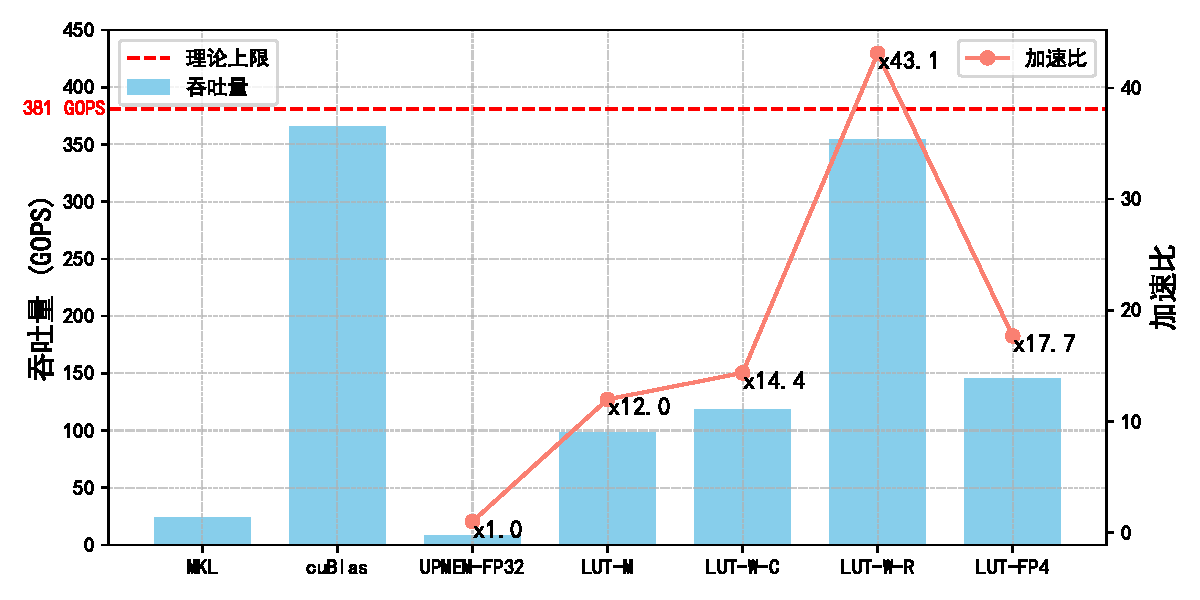
\includegraphics[width=0.9\textwidth]{figures/Exp1-1.pdf}
    \caption{不同平台及算法下GEMV总吞吐}
	\label{EXP1-1}
\end{figure}

结果显示,与CPU平台的MKL库中的矩阵向量乘法相比,UPMEM平台的最大吞吐算法LUT-W-R算法有14.7倍的提升,而相比较GPU的cuBlas而言,吞吐量基本持平有微小的差距。CPU平台使用MKL库充分利用了Intel CPU的向量指令和多线程(OpenMP,设置线程数量为16)并行计算,但是由于CPU平台有限的内存带宽和复杂的存储层级,GEMV受到数据传输的限制,性能与近存计算平台相差较大。对于GPU的表现符合预期,因为GPU的内部带宽并不低,此前在第四章的分析中发现UPMEM平台的内存带宽利用率最高也只达到10\%左右,因此二者在数据传输方面的表现是类似的。同时GPU的核心数量并不少,且每个核心的主频更是有1.41GHz是UPMEM的核心主频的2~3倍,因此理应相较于UPMEM更快,但是UPMEM平台凭借着高速的内部带宽和精调的优化算法缩小了与GPU平台的差距。同时在GPU测试的过程中,我们发现计算吞吐(Compute SM Troughput)仅达47.57\%,远远没有充分利用硬件计算的能力,然而内存带宽利用率却以及达到96.89\%表现为内存瓶颈。

同时可以看到在UPMEM平台上,软件优化的加速比。以最基础的GEMV算法UPMEM-FP32为基准,该算法就是普通地使用UPMEM上的软件模拟Float32直接进行计算而不采用查找表,其性能非常低,吞吐仅达8GOPS。使用了针对MRAM的分块载入查找表的算法LUT-M后,相比UPMEM-FP32有巨大的提升,加速比高达12倍。之后是针对WRAM优化的两种算法将矩阵行重排LUT-W-R和矩阵列重排LUT-W-C。在这之中,LUT-W-C的算法的提升有限,达到UPMEM-FP32的14.4倍,而LUT-W-R算法提升较高,是各种软件优化算法中吞吐最高的算法,达到355GOPS,是UPMEM-FP32的43.1倍。LUT-FP4的算法是卸载W4A8量化的矩阵向量乘法,因为权重进一步量化到了4bit,因此乘法查找表的大小刚好只有16KB,完全能够放在WRAM中,因此执行的算法与UPMEM-FP32是类似的,同样是矩阵向量的内积,只不过乘法换成了查表操作。此处比较奇怪的是,LUT-FP4算法虽然相比UPMEM-FP32算法有17.7倍的提升,但是却弱于LUT-W-R算法,而LUT-W-R算法是载入子矩阵同样进行内积操作,理应比LUT-FP4要更慢。我们通过研究两种算法的汇编代码后发现,LUT-W-R的算法汇编代码进行了循环展开而LUT-FP4完全没有展开,换言之LUT-W-R的编译优化非常好,性能远超LUT-FP4(在第三小节的测试也侧面说明了这一点),因此出现了LUT-FP4算子吞吐弱于LUT-W-R的情况,推测主要原因在于UPMEM的软件栈不够完善。

同时为了评估硬件限制对UPMEM平台的影响,将LUT-W-C算法下的GEMV的实际性能与理论性能进行了比较。理论性能通过公式\ref{MaxThroughput}计算。其中$N_{dpu}$表示 UPMEM核心的数量,为2560。$F$表示核心频率,为400MHz。$N_{inst}$表示执行一次FMA操作所需的指令数,包括5条指令:1条用于加载权重,1条用于地址生成,1条用于乘法,1条用于加法,以及1条用于循环中的杂项操作。理论带宽上限为381GOPS,测试的LUT-W-C算法的GEMV算子吞吐为355GOPS,大概达到理论性能的93\%。

\begin{equation}
    MaxThroughput=\frac{2\times N_{dpu}\times F}{N_{inst}}\; GOPS
    \label{MaxThroughput}
\end{equation}

\subsection{能效比测试与瓶颈分析}
近存硬件平台的一大优势在于其减少了数据移动的开销从而能够更加节能,非常适合边端对功耗有严格要求的设备,因此我们在测试计算能力的同时也测试了各个硬件平台的能效比。我们使用Intel VTune Profiler来测试CPU平台上的能耗,同时使用Nsight工具来测试GPU平台的能耗。对于UPMEM平台,由于官方没有提供能耗测试工具,因此我们只能通过UPMEM SDK的dpu-diag工具测试DPU的内核和DRAM Bank的静态功耗,大约为12.8w每根DIMM条。能效比定义简单地计算公式为\ref{EnergyEffiency},其中算子吞吐与上一小节中的测试结果保持一致,Energy为能耗,单位瓦特(W)。

\begin{equation}
    EnergyEffiency=\frac{Troughput}{Energy}\; GOPS/W
    \label{EnergyEffiency}
\end{equation}

能效比的实验如图\ref{EXP1-2:1}所示,其中以CPU平台的能效比作为基准(1),对其他平台和算法的能效比进行了测试和数据整理,可以看到除了UPMEM-FP32算法因过低的算子吞吐导致能效比较低外,其他平台的能效比皆高于CPU平台,其中最高能效比的算法为LUT-W-R,是CPU平台的8.6倍,是GPU平台的1.13倍,结果充分显示了近存计算平台的低能耗的优势。

\begin{figure}[htbp!]
	\centering
	\subfigure[能效比实验]{
		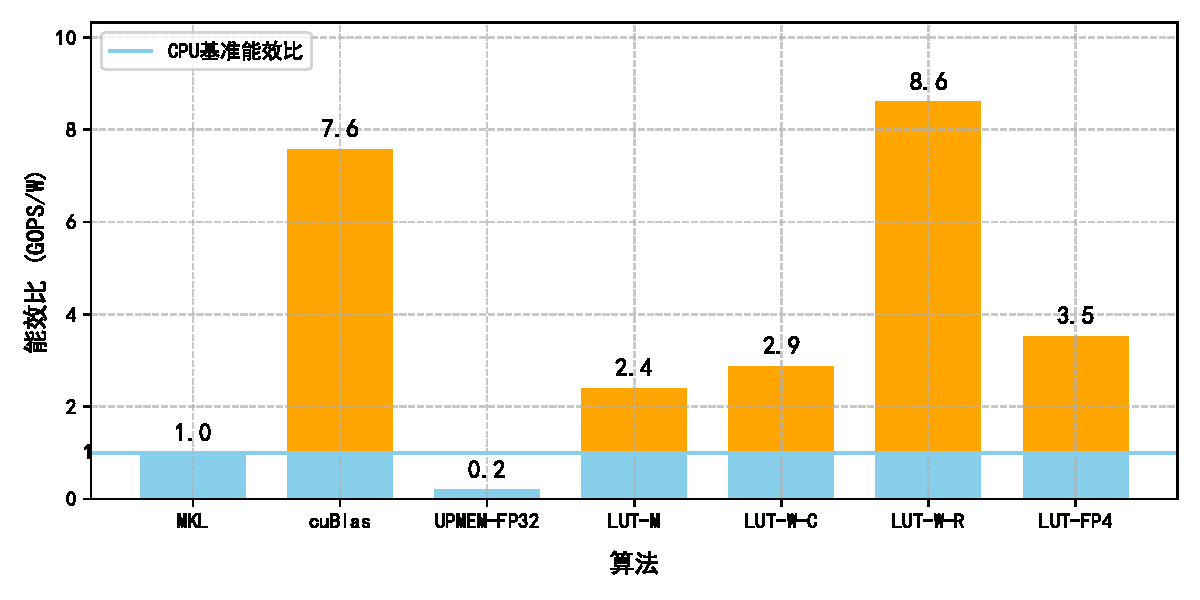
\includegraphics[width=0.9\linewidth]{figures/Exp1-2-1.pdf}
		\label{EXP1-2:1}}
	\\
	\subfigure[瓶颈分析]{
		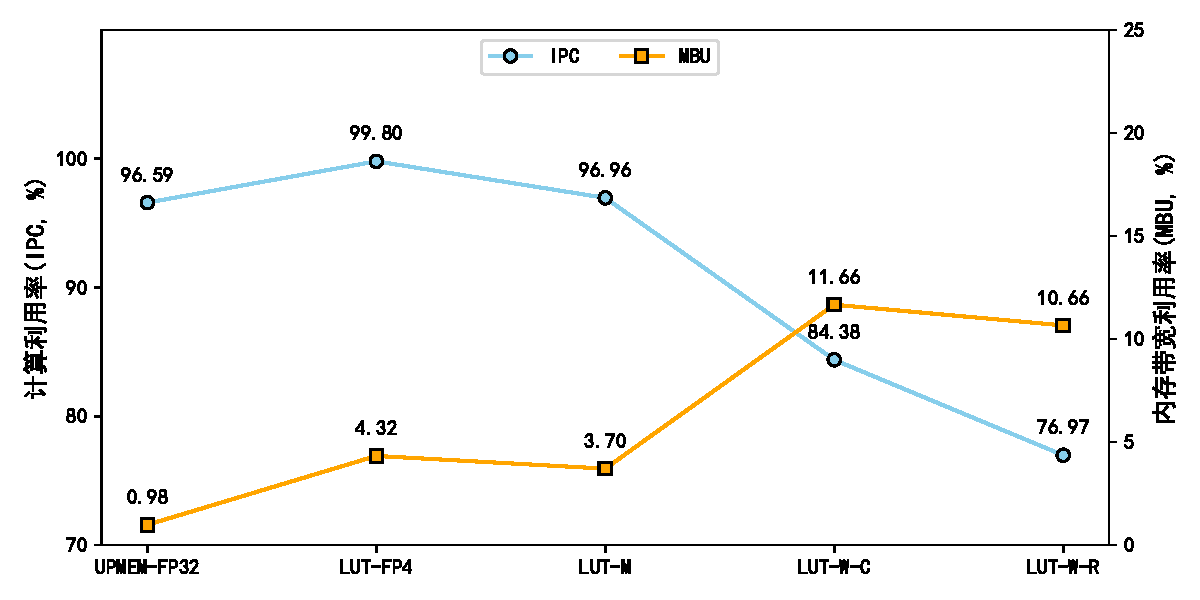
\includegraphics[width=0.9\linewidth]{figures/Exp1-2-2.pdf}
        \label{EXP1-2:2}}
	\caption{不同平台及算法下GEMV能效比和瓶颈分析}
	\label{EXP1-2}
\end{figure}

同时在这里对第四章的表\ref{BottleneckTable}进行补充测试,完善了UPMEM平台下各种算法的计算利用率和内存带宽利用率的数据如图\ref{EXP1-2:2}所示,此时矩阵的大小为$4096\times 4096$,设置16个Tasklets,LUT-W-R算法配置子矩阵大小为$32\times 64$。此前已分析过CPU平台和GPU平台都是内存瓶颈,反观UPMEM平台的各种算法,IPC都相当之高而内存带宽利用率仅最高达11\%,是非常明显的计算瓶颈的表现。同时可以看到逐步优化算法会将IPC降低而MBU提高,是非常典型的使用访存减少计算的优化手段,这意味着在UPMEM这种近存平台编程或者加速应用需要转变此前的冯诺依曼架构计算机的编程定式——减少访存,在近存平台上访存变得更加的“便宜”,我们往往需要用访存换计算。

此外实验中比较特殊的点在于LUT-FP4相较于LUT-M,从MRAM读写的字节数量是相同的(FP4仍然用8bit存储减少取数的开销),但是由于LUT-FP4能够执行GEMV内积而LUT-M只能执行GEMV外积导致LUT-FP4的WRAM访问更少,因此运行时间更短,IPC更高且MBU更高。

\subsection{扩展性测试}
本小节将从两个方面对算法进行扩展性测试,首先测试UPMEM每个DPU中的多线程扩展性,即保持矩阵的尺寸不变,增多Tasklet数量,观察算法性能。另一个方面,我们将测试算法处理矩阵尺寸的扩展性,即保持Tasklet的数量不变,增大矩阵的尺寸观察算法的性能。

对于多线程扩展性,本小节测试的矩阵大小为$4096\times 4096$,具体的算法选择以下几种:UPMEM-FP32,LUT-FP4,LUT-M,LUT-W-C,LUT-W-R。设置Tasklet数量从1逐渐翻倍到16,测试各个算子的执行时间如图\ref{EXP3-1}所示。可以看到无论是哪种算法,随着Tasklet的成倍增加,各个算法的执行时间随之成倍减少(对数坐标),然而当Tasklet的数量从8变化到16时,执行时间只减少到了原来的1.3倍,这个刚好符合从8变化打11扩大1.3倍的数据对应关系,也同样验证了UPMEM的流水线在11个线程时就已经充满,多增加线程无继续提升计算吞吐的硬特性。

\begin{figure}[htbp]
    \centering
    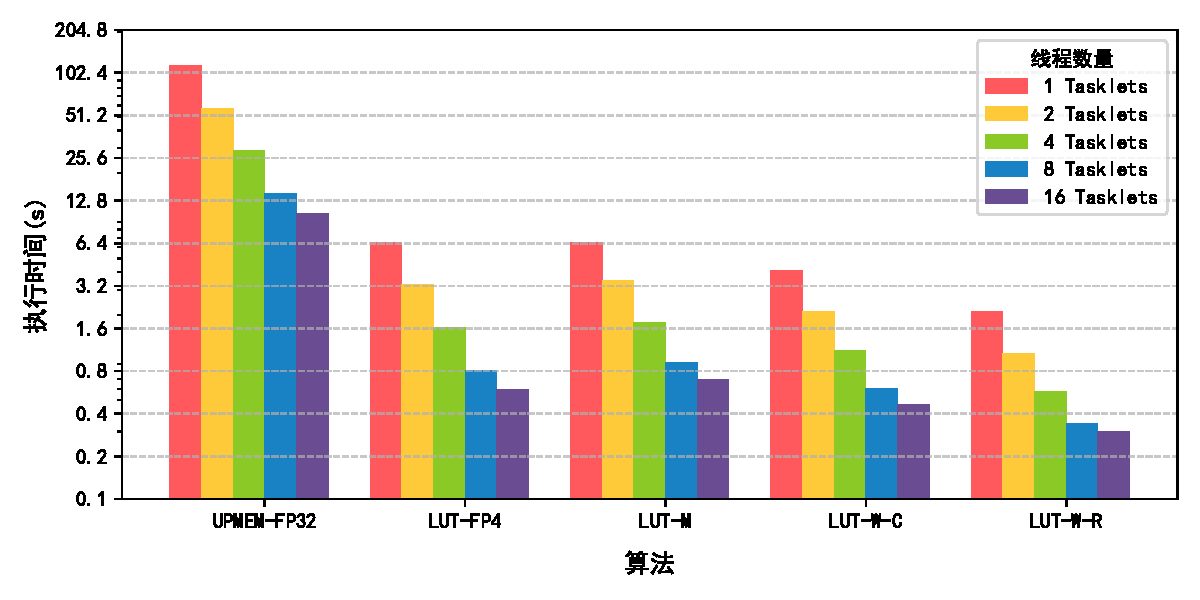
\includegraphics[width=0.9\textwidth]{figures/Exp3-1.pdf}
    \caption{UPMEM平台不同GEMV算法的多线程扩展性测试}
	\label{EXP3-1} %% label for entire figure 
\end{figure}

在Llama2-7B的MHSA中,会将一个完整的4096长度的词向量通过线形层成映射到32个子空间,对应到32个头(会将$4096\times 1$的向量映射成32个$128\times 1$的向量),本质上属于降维操作,(单个头)线形层是一个$4096\times 128$的窄矩阵;在最终计算得到attention向量后,又会通过一个线性层将$128\times 1$的向量重新映射为$4096\times 1$并最终合并各个头的结果,属于升维操作,此时线形层是一个$128\times 4096$的宽矩阵。同时由于DPU的通信开销低的特性,往往对算子进行融合,比如将QKV的单个头的线性层合并为大矩阵,此时的维度就是$4096\times 384$,且MLP部分的矩阵可以随意切分,因此在实际的大模型推理过程中会遇到不同尺寸的矩阵。此前受制于多个平台的内存容量问题,我们只测试了$4096\times 128$的矩阵性能,当矩阵的行列发生变化时,算法的性能是否能够随之正常扩展,这是影响推理效率的关键问题。

对于矩阵尺寸扩展性测试,同样选择UPMEM-FP32,LUT-FP4,LUT-M,LUT-W-C,LUT-W-R这几种算法,设置Tasklet数量为16,改变工作负载,将矩阵的尺寸从$4096\times 256$翻倍变化到$4096\times 4096$,同样将$256\times 4096$翻倍变化到$4096\times 4096$,测试各个算子的执行时间如图\ref{EXP3-2}所示。

对于改变矩阵的行数来说,如图\ref{EXP3-2:2},成倍地将矩阵的行数从128翻倍到4096,算子的执行时间基本上是成倍地增加,说明上述的算法对于矩阵的行变化并不敏感。对于改变矩阵的列数来说,如图\ref{EXP3-2:1},同样的翻倍手段,大部分算法都是符合成倍减少的特性,对列变化不敏感,只有LUT-M和LUT-W-C除外。这两个算法对于列的成倍增加,算法的执行时间并未成倍的增加,而是低于2倍地增加,换句话说,当成倍减少矩阵的列时,LUT-M和LUT-W-C的算法反而会“耗时增加”。

其中的原因在于这两个算法都是以行为单位进行同步和计算的,LUT-M和LUT-W-C每次会载入权重矩阵的一行,当列数变小时,因MRAM的DMA引擎的特点(大批量数据载入带宽更高),DMA的效率就会变低,相对应的执行时间就会变多。同时LUT-W-C的算法的优化的理论在于矩阵一行的所有元素不必都查一次表而只需查256次,即通过减少查表的次数来减少访存。当列数变小时,甚至小于256时,LUT-W-C的查表次数反而可能超过未经过优化的查表次数,因此相比于LUT-M,LUT-W-C的“耗时增加”会更严重。

\begin{figure}[htbp!]
	\centering
	\subfigure[固定列为4096改变矩阵行]{
		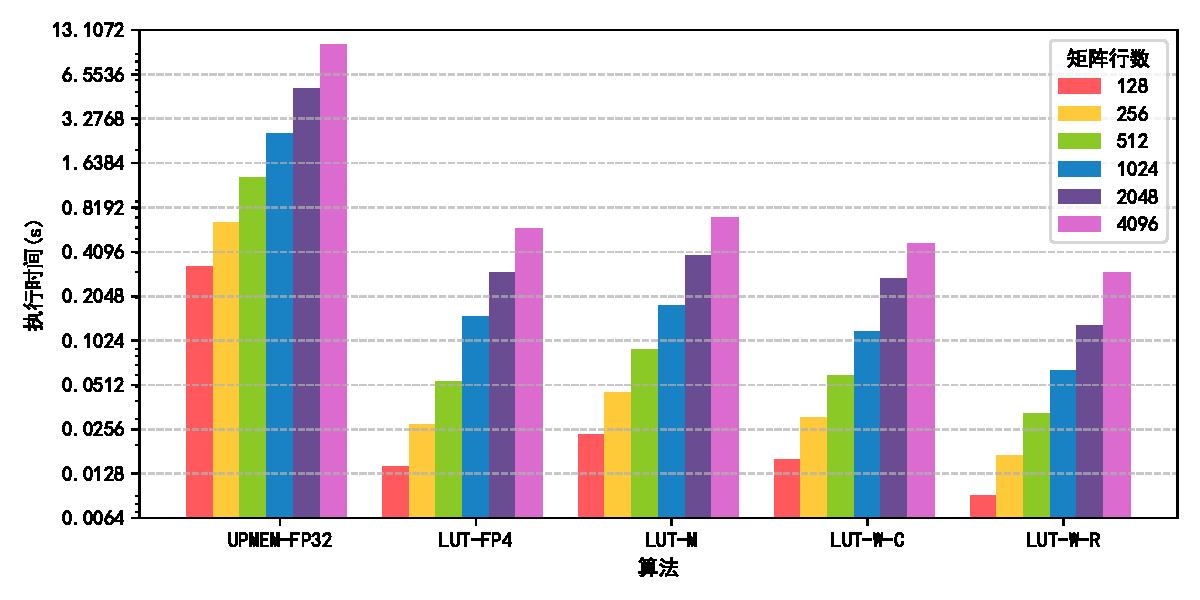
\includegraphics[width=0.45\linewidth]{figures/Exp3-2-2.pdf}
        \label{EXP3-2:2}}
	\subfigure[固定行为4096改变矩阵列]{
		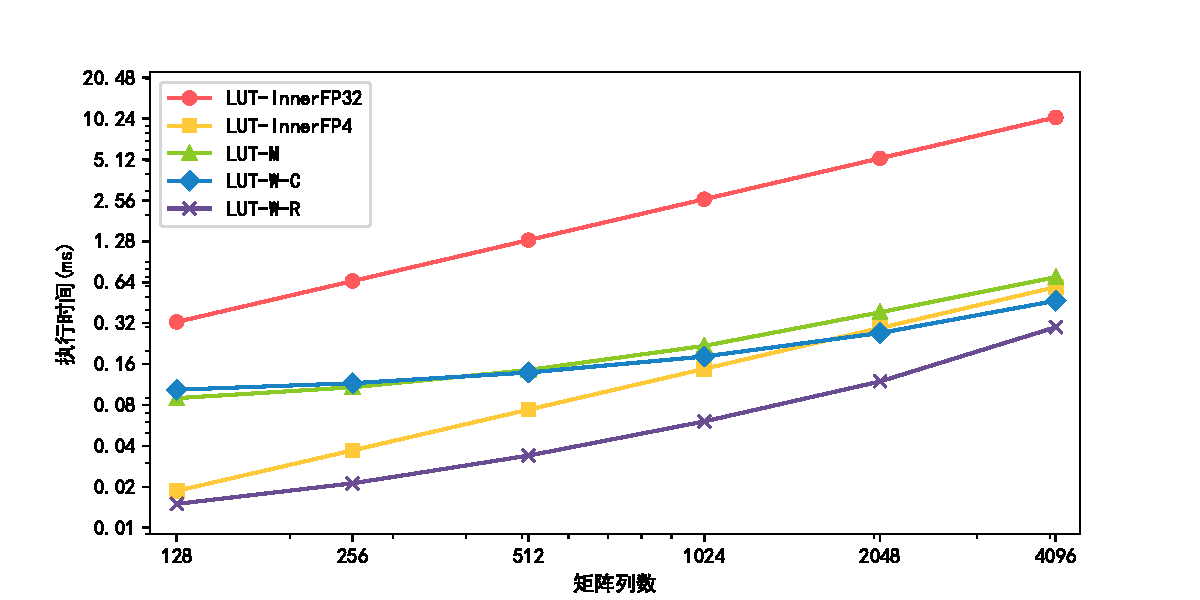
\includegraphics[width=0.45\linewidth]{figures/Exp3-2-1.pdf}
		\label{EXP3-2:1}}
	\caption{UPMEM平台不同GEMV算法矩阵尺寸扩展性测试}
	\label{EXP3-2}
\end{figure}

此外可以看到LUT-W-R在增加矩阵的列时,其执行时间并不是等比增长,而是耗时越来越多,原因在于LUT-W-R算法本身对权重矩阵的行列并不敏感,而是对其分块处理的子矩阵的大小敏感,子矩阵越大执行耗时越少。当增加矩阵的列时,会较为严重地挤占WRAM的空间导致子矩阵的变小,从而需要更多的DMA操作从MRAM中读取数据,从而造成执行耗时增加因此可以得出结论,LUT-W-R的算法更加适合行数远大于列数的“窄矩阵”,而LUT-W-C的算法更加适合列数远大于行数的“宽矩阵”。

\section{基于模拟器平台的硬件设计测试与分析}
在真实硬件平台测试后GEMV算子的各项数据后,需要对基于模拟器平台的硬件优化进行测试。我们分别做了两部分的硬件优化,分别是增加了融合查表加法指令集(FLA)和向量指令(SIMD):使用FLA指令优化第三章提出的三个基于查表的算法LUT-M、LUT-W-C和LUT-W-R;使用SIMD指令优化GEMV朴素内积LUT-FP4的算法LUT-SIMD。基于UPMEM周期精确模拟器PIMulator对上述优化进行测试,通过模拟器模拟器的周期数和主频测算算子执行耗时,进而得到算子优化后的吞吐。设置矩阵的尺寸为$4096\times 4096$,设置16个Tasklets,LUT-W-R算法配置子矩阵大小为$32\times 64$。具体的加速如图\ref{EXP2-1}所示。

\begin{figure}[!htbp]
    \centering
    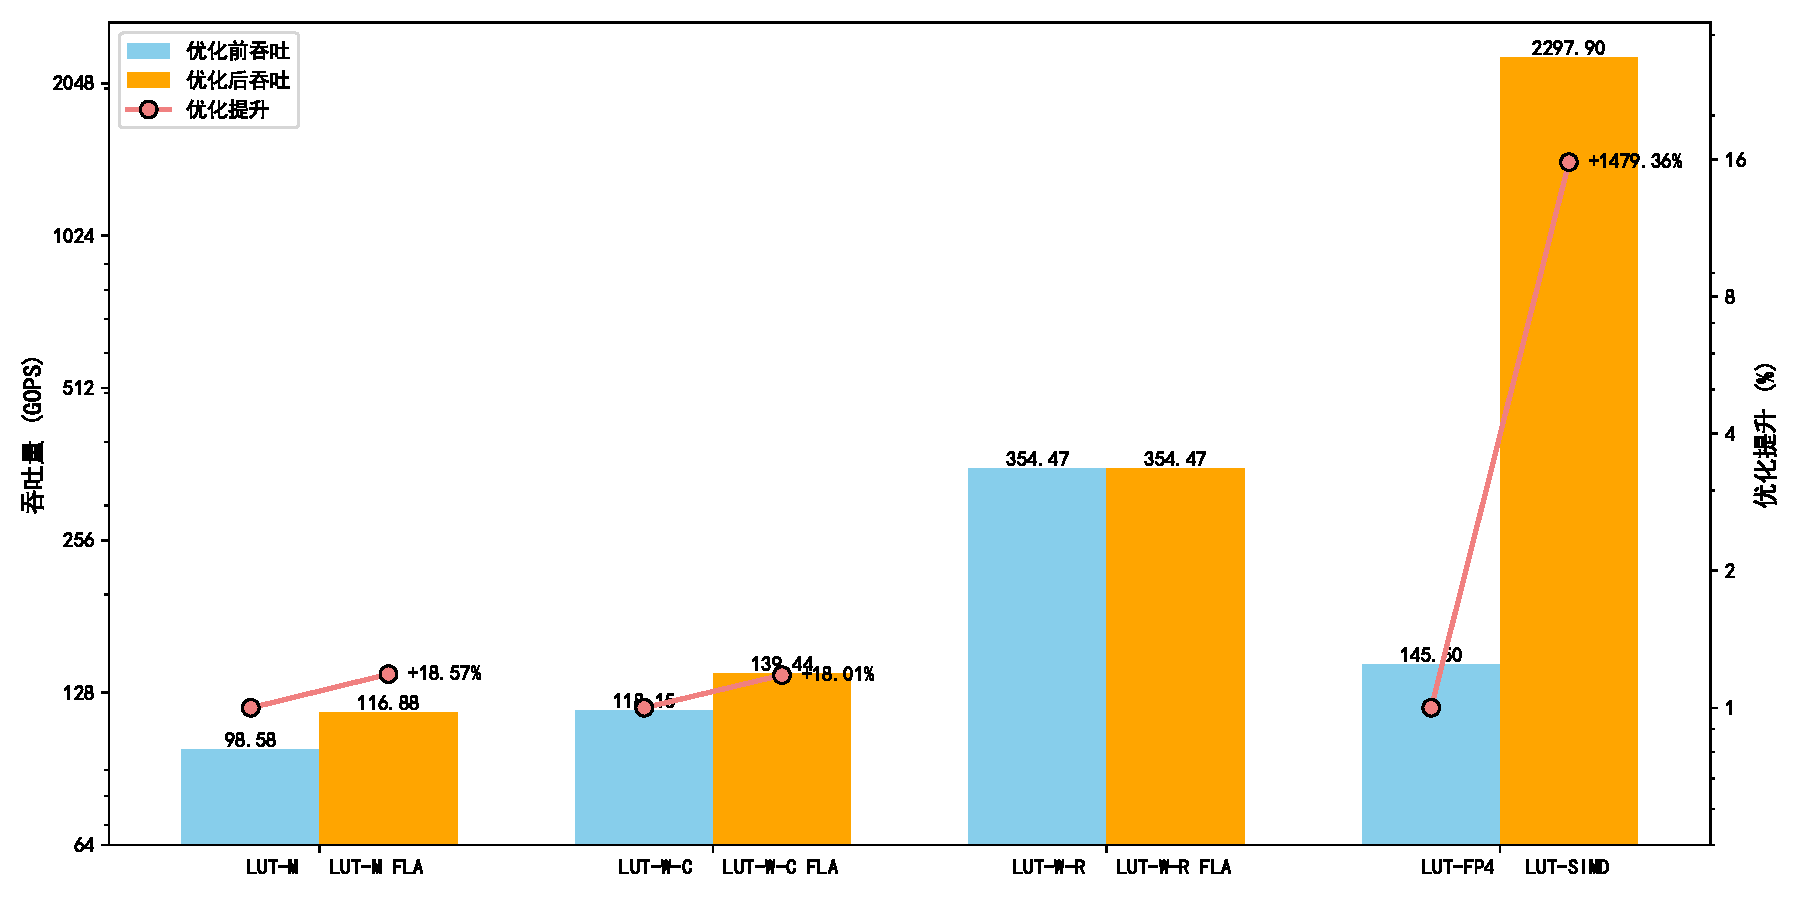
\includegraphics[width=0.9\textwidth]{figures/Exp2-1.pdf}
    \caption{硬件架构修改对于GEMV算子吞吐提升——编译优化O3}
	\label{EXP2-1}
\end{figure}

对于算法LUT-M、LUT-W-C和LUT-W-R而言,使用了FLA指令集后算子的吞吐提升分别在14.88\%、27.82\%和0\%,在这里对结果进行解释。对于LUT-M和LUT-W-C而言,提升大概在15\%~30\%左右较为优秀但是没有达到理论预期。在汇编分析的代码段\ref{LUTInstAsm}中,FMA操作的提升普遍在2~3倍,但是上述假设的情况过于理想,没有考虑寄存器的使用限制以及编译优化手段,在真实的算法汇编代码中,能够使用我们设计的查找指令的代码段仅仅在查表指令代码段一处,并且通过一定的编译优化对指令进行了重排,无法通过人手动地更改整体代码段以达到最佳优化,其结果就是使用我们设计的FLA指令往往只能优化FMA操作中的一条到两条指令:比如LUT-M仅有一处查表可以使用FLA指令增强,就是最深循环出的查表语句;而LUT-W-C算法有两处可以使用FLA指令增强,一处是查表得乘积,另一处是查表得累加索引。而我们在之前的理论最大算子吞吐的计算过程中展示过,理论上一次FMA操作往往需要消耗5条指令,因此优化大概在15\%~30\%左右符合预期。

对于算法LUT-W-R而言,我们无法通过汇编代码分析找到任何可以优化的代码段。我们分析发现LUT-W-R的算法编译优化非常好,将查表操作的额外开销部分通过指令重排优化掉了,从而导致我们无法直接从汇编代码入手优化算法,因此并无加速效果。从上面的测试可以看出,UPMEM平台的软件生态较为完善,编译优化较好,其中的部分原因可能是UPMEM本身基于RISC指令集,本身指令简单且优化成熟。然而很多其他的近存计算平台,由于底层的硬件和支持的指令集并不像UPMEM这样简单且流行,仍然存在不完善的软件链,编译优化不好的问题。因此基于上面的实验,我们做了补充实验\ref{EXP2-2},对于各个算法不开启编译优化,其余配置保持一致测试了结果。

\begin{figure}[!htbp]
    \centering
    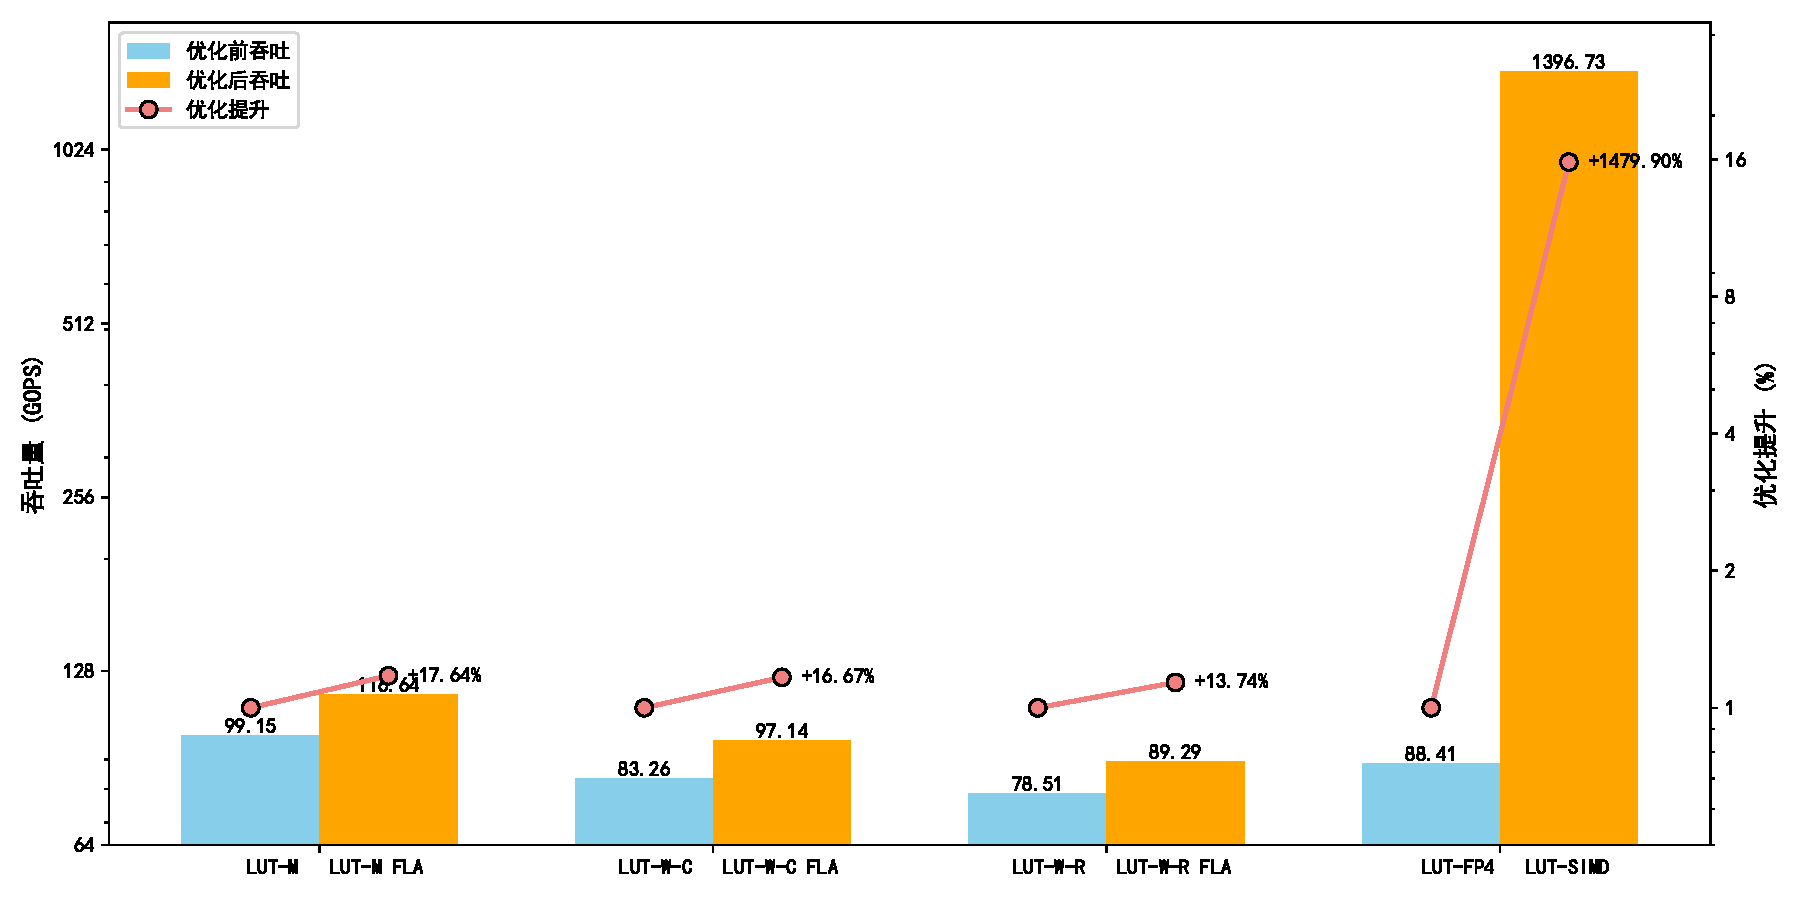
\includegraphics[width=0.9\textwidth]{figures/Exp2-2.pdf}
    \caption{硬件架构修改对于GEMV算子吞吐提升——编译优化O0}
	\label{EXP2-2}
\end{figure}

这时对于算法LUT-M,使用了FLA指令集后算子性能提升能达到17.64\%,有少许提升。算法LUT-W-C的提升为16.67\%,该算法的FLA指令增强和O3编译一样有两处,但是提升反而相比于O3编译减少了,其原因在于LUT-W-C的未经编译优化其复杂的源码结构使得其编译产生的汇编代码非常低效,吞吐量甚至低于LUT-M(LUT-W-R也是类似),并且我们在编译的汇编指令中发现了许多废指令,我们未将这些废指令或非查找表的指令优化计入,因此整体LUT-W-C的提升变低了。LUT-W-R此时就有了13.74\%的提升,提升较低的原因和其总吞吐低有关。

可以看到,对于编译优化较差的平台我们的FLA指令增强效果较好,尤其对于算法LUT-W-C,有两次随机数组访问(查表),优化效果是最好的。但是我们提出的一系列FLA指令集其实不止局限于查表的优化,可以用于多种场景,许多移位、访存和累加操作都可以通过一条FLA指令完成。此时的工作应该在编译器层面进行,直接进行汇编指令的替换不会有效果。

对于使用SIMD指令加速的效果,不论编译优化等级,比较LUT-FP4和LUT-SIMD可以发现,加速效果约为16倍(提升是1479\%差不多就是原来的16倍),这与理论提升高度符合,因为可以一次性向量完成16个元素的查表和加法,同时我们简单地修改了PIMulator模拟器的让其支持向量指令且保证CPI(Cycle Per Instruction)为1,与其他的RISC指令并无明显差异,因此原本16个元素的计算需要16次载入激活、载入矩阵、查表、累加,而使用向量指令后,就变成了1次载入子表、矩阵向量移位、重排、累加(每8次操作载入一次矩阵向量),因此性能提升非常大。

当然我们在模拟器上实现时并未考虑实际的硬件工艺和电路设计是否允许这样的支持,比如是否能够在较小的芯片内集成支持512bit向量计算的向量单元,并且能支持指令的CPI达到1。当然我们可以结合更低bit权重量化的工作减小向量的长度,比如3bit的权重量化只需要256bit的向量运算,而2bit只需要128bit。

在真实硬件平台上测试的能效比、瓶颈分析和扩展性实验,在模拟器平台上测试结论基本保持一致,在此不多赘述。

\section{本章小结}
本章对此前的软硬协同优化方案做了充分的测试及结果分析。首先介绍了测试的环境和基本配置,包括所使用的三大硬件平台的基本介绍和硬件配置,测试数据的配置以及对比基线的设置。然后在商用近存计算硬件UPMEM上做了一些的测试和分析,包括对各种基于UPMEM的优化算法的GEMV算子总吞吐测试,对比了CPU和GPU平台的算子吞吐,分析得到结论:UPMEM上GEMV算子强于CPU平台并于GPU平台持平;同时包括对三个硬件平台GEMV计算的能效比测试以及计算瓶颈分析,分析得到近存计算平台UPMEM的能效比高于CPU和GPU平台且GEMV的优化算法表现为计算瓶颈;还包括对GEMV算子的扩展性测试,测试得到此前提出的GEMV算法对于Tasklet有良好的扩展性(不超过11个线程),而对于矩阵的尺寸大多也同样具有良好的扩展性,其中LUT-M和LUT-W-C算法更适合在行数远小于列数的矩阵,而LUT-W-R则更适合行数远大于列数的矩阵。最后在PIMulator模拟器上测试硬件的修改对于GEMV算子性能的提升,其中增加FLA指令集对于LUT-M和LUT-W-C的提升在15\%~30\%左右,增加向量处理单元对于LUT-FP4算法的提升在16倍。
% \chapter{总结与展望}
\section{总结}
\section{展望}%要插入本科签名的最后一个章节,插入命令使用\input{}
\chapter{总结与展望}
\section{总结}
\section{展望}%要插入本科签名的最后一个章节,插入命令使用\input{}

%本科签名
%\autograph


%参考文献
% \cleardoublepage
\phantomsection % 手动设置书签锚点
\addcontentsline{toc}{chapter}{参考文献}
\printbibliography


% %附录
% \appendix
% \chapter{如何正确安装\LaTeX\ }

Noun–verb dependencies in various languages and their biological ana- logues. Part A) shows the sentence “Dick saw Jane help Mary draw pictures” trans- lated grammatically into German and Dutch. That is, the words in the sentence are rearranged to reflect the rules of grammar in these two languages, but the sentence is not translated per se. As shown, the English version of the sentence has a rela- tively simple dependency structure between the nouns and verbs that can be modeled using regular grammars. In contrast, German and Dutch require more complicated grammatical models . Part B) shows the biological analogue of the three sen- tences in Part A). Typically, restriction sites can be modeled using regular grammars, whereas complex DNA secondary structures require context–free or context–sensitive grammars . In the first example, the arches are used to represent a “must be followed by” dependency. In the second two examples, they represent a “must be complementary to” dependency.


%致谢
\begin{acknowledge}%致谢
时光荏苒,两年的专业硕士学习生涯即将画上句号,在这段旅程的终点,我心中满是感恩,千言万语如潮水般涌上心头。

我要将最诚挚的敬意与感谢献给我的指导老师王晶教授。从论文选题时的迷茫与徘徊,到构思阶段的反复斟酌,再到撰写过程中的字斟句酌,直至最终定稿的每一个细节,王老师都给予了我悉心的指导和耐心的帮助。她严谨的治学态度,体现在对每一个数据、每一处引用的严格把关;她渊博的学术知识,犹如一座取之不尽的宝库,总能在我困惑时提供多元的思路;她精益求精的工作作风,更是深深烙印在我的心中,激励着我不断追求卓越。当研究陷入瓶颈,数据出现偏差,思路陷入僵局时,王老师总是能以其敏锐的洞察力,迅速发现问题的关键所在,为我指明前行的方向,用温暖而坚定的话语鼓励我坚持下去。她不仅是我学术道路上的引路人,在生活中,她的为人处世、对待困难的从容态度,也成为我人生路上的榜样,让我深刻领悟了为学与为人的真谛。回首这段历程,若没有王老师的指导与支持,我绝不可能顺利完成这篇毕业论文。

在实验室的日子里,师兄师弟们也给了我莫大的帮助。初入实验室时,面对复杂的机器环境和复杂的操作流程,我满心茫然。师兄们凭借丰富的经验,手把手地教我科研,从选题的发现、文献的调研,到实验步骤的具体实施,每一个环节都耐心示范。他们还毫无保留地分享自己的研究心得,讲述曾经遇到的问题及解决方法,让我少走了许多弯路。师弟们积极向上的态度和对科研的热情,也时刻感染着我。在实验紧张忙碌时,大家相互打气;在数据出现异常时,一起查阅资料、分析原因。我们围坐在实验台前,激烈讨论研究方案,那些一起在实验室忙碌的日夜,不仅充实了我的知识储备,更让我收获了珍贵的友谊。

而家人,始终是我最坚实的后盾。我的母亲,在生活中给予我无微不至的关怀。清晨,她早早起床准备营养丰富的早餐;夜晚,当我还在书桌前埋头苦读时,她会悄悄端来一杯热牛奶。家中的大小事务,她默默承担,从不让我操心,让我能够心无旁骛地专注于学业。每当我遇到挫折情绪低落时,母亲总是用温暖的话语安慰我,回忆我过往取得的成绩,鼓励我重新振作。她的坚韧与乐观,一直潜移默化地影响着我,是我不断前进的动力源泉。

在未来的日子里,我会带着这份感恩,将所学用于实践,不辜负所有给予我帮助的人。愿王老师的教诲如春风化雨,培育出更多优秀的学子,桃李满天下;愿实验室的伙伴们在科研道路上,能突破重重难关,一帆风顺;愿家人平安健康,岁月温柔以待。
    
\end{acknowledge}



\end{document}  
